\documentclass[11pt,reqno]{amsart}
\usepackage[top=1in, left=1in, right=1in, bottom=1in]{geometry}
\geometry{letterpaper}                   % ... or a4paper or a5paper or ...

\usepackage[parfill]{parskip}    % Activate to begin paragraphs with an empty line rather than an indent
\usepackage{algorithm}
\usepackage{algpseudocode}
\usepackage{hyperref}
\usepackage{url}
\usepackage{verbatim}
\usepackage{amssymb}
\usepackage{amsmath}
\usepackage{enumitem}
\usepackage{setspace}
\usepackage{natbib}
\usepackage{algpseudocode}
\usepackage{graphicx}
\usepackage{times}

%\usepackage{epstopdf}
%\DeclareGraphicsRule{.tif}{png}{.png}{`convert #1 `dirname #1`/`basename #1 .tif`.png}

\newcommand{\RR}{I\!\!R} %real numbers
\DeclareMathOperator{\diag}{diag}

\algnewcommand{\Inputs}[1]{%
  \State \textbf{Inputs:}
  \Statex \hspace*{\algorithmicindent}\parbox[t]{.8\linewidth}{\raggedright #1}
}
\algnewcommand{\Initialize}[1]{%
  \State \textbf{Initialize:}
  \Statex \hspace*{\algorithmicindent}\parbox[t]{.8\linewidth}{\raggedright #1}
}

\title[VI for RVD]{Variational inference for rare variant detection in deep, heterogeneous next-generation sequencing data}
\author[F. Zhang]{Fan Zhang}\address{Department of Biomedical Engineering, Worcester Polytechnic Institute}
\author[P. Flaherty]{Patrick Flaherty}\address{Department of Mathematics and Statistics, University of Massachusetts, Amherst}

\begin{document}

\maketitle

\begin{abstract}
  The detection of rare variants is important for understanding the genetic heterogeneity in mixed samples.
Recently, next-generation sequencing (NGS) technologies have enabled the identification of single nucleotide variants (SNVs) in mixed samples with high resolution.
Yet, the noise inherent in the biological processes involved in next-generation sequencing necessitates the use of statistical methods to identify true rare variants.
We propose a novel Bayesian statistical model and a variational expectation-maximization (EM) algorithm to estimate non-reference allele frequency (NRAF) and identify SNVs in heterogeneous cell populations.
We demonstrate that our variational EM algorithm has comparable sensitivity and specificity compared with a Markov Chain Monte Carlo (MCMC) sampling inference algorithm, and is more computationally efficient on tests of low coverage (27$\times$ and 298$\times$) data.
Furthermore, we show that our model with a variational EM inference algorithm has higher specificity than many state-of-the-art algorithms.
In an analysis of a directed evolution longitudinal yeast data set, we are able to identify a time-series trend in non-reference allele frequency and detect novel variants that have not yet been reported.
Our model also detects the emergence of a beneficial variant earlier than was previously shown, and a pair of concomitant variants.
\end{abstract}

\section{Introduction}
Massively parallel sequencing data generated by next-generation (NGS) technologies is routinely used to interrogate SNVs in research samples ~\citep{koboldt2013next}.
For example, deep sequencing confirmed the degree of genetic heterogeneity of HIV \citet{} and influenza ~\citep{flaherty2011ultrasensitive}.
Many solid tumors are represented as having intra-tumor heterogeneity by DNA sequencing technology, where SNVs are rare in the population ~\citep{navin2010inferring}.
Also, whole genome sequencing has revealed that many beneficial mutations of minor allele frequencies are essential to respond to dynamic environments ~\citep{kvitek2013whole}.
However, rare SNVs identification in heterogeneous cell populations is challenging, because of the intrinsic error rate of next generation sequencing platform ~\citep{shendure2008next}.
Thus, there is a need for accurate and scalable statistical methods to uncover SNVs in heterogeneous samples.

% Classes of Methods %
% Probabilistic methods: Bayesian %
A number of computational methods have been developed to detect SNVs in large scale genomic data sets.
These methods can be roughly categorized as probabilitic or heuristic or some combination.
Among all of the current probabilistic methods, the Bayesian probabilistic framework has been increasingly used to calculate the unobserved quantities such as variant allele frequency given the observed genomic sequencing data.
GATK ~\citep{mckenna2010genome} and SAMTools ~\citep{li2009sequence} use a naive Bayesian decision rule to call variants.
EBCall models sequencing errors based on a Beta-Binomial distribution, where the parameters and latent variables are estimated from a set of non-paired normal sequencing samples ~\citep{shiraishi2013empirical}.
However, the error rate of normal sequencing samples could be unmatched with the error rate of the target samples, which may cause a problem of making false negatives calls ~\citep{wang2013detecting}.
CRISP compares aligned reads across multiple pools to obtain sequencing errors, and then distinguishes true rare variants from the sequencing errors ~\citep{bansal2010statistical}.
However, the bottleneck of CRISP is its low computational efficiency due to a calculation of a large amount of contingency tables.
% Other Bayesian methods: MAQ, Mutect, and FamSeq

% Joint distribution %
Generally, independent modeling method models the genotypes of tumour and normal samples separately and then looks for the difference between them.
In contrast to independently analyzing a tumour-normal pair, joint modeling method models a joint-genotype of the tumour and normal samples simultaneously.
JointSNVMix introduces two Bayesian probabilistic models (JointSNVMix1 and JointSNVMix2) to jointly analyze a tumour-normal paired allelic count of NGS data ~\citep{roth2012jointsnvmix}.
JointSNVMix derives an expectation maximization (EM) algorithm to calculate maximum a-posteriori (MAP) estimate of latent variables in a particular probabilistic graphical model.
Furthermore, \citet{roth2012jointsnvmix} reveals that the joint modeling method, JointSNVMix1, observes 80-fold reduction of false positives compared with its independent analogue (SNVMix1).
SomaticSniper ~\citep{larson2012somaticsniper} models the joint diploid genotype likelihoods for both tumour and normal samples.
Additionally, Strelka \citet{saunders2012strelka} models the joint probabilistic distribution of allele frequencies for both tumour and normal samples, which is demonstrated to be more accurate compared with the methods based on the estimated allele frequency tests between tumour and normal samples.

% Frequentist %
SNVer focuses on a frequentist method that is able to calculate $P$-values, but the author pointed out that this approach fails to model sampling bias that will reduce the power of detecting true rare variants ~\citep{wei2011snver}.

% Heuristic %
An alternative strategy to probabilistic methods are heuristic methods, use a set of criteria to select variant positions instead of modeling the data using probabilistic distributions.
%By setting thresholds of the rules, heuristic algorithms can find a good solution, but optimum is not guaranteed.
VarScan is an example of a heuristic method that compares tumour and normal samples by satisfying some lower bounds, such as a certain variant allele frequency and a number of allele counts ~\citep{koboldt2012varscan}.
%VarScan is based on Fisher's exact test to estimate sample allele frequencies.

% RVD2 %
In previous work, we developed a Beta-Binomial model to characterize a null hypothesis error rate distribution at each position.
Using this, we call rare variants by comparing the error rate of the sample sequence data to a null distribution obtained from sequencing a known reference sample ~\citep{flaherty2011ultrasensitive}.
RVD can identify mutant positions at a 0.1\% fraction in mixed samples using high read depth data.

We improved upon that work in, RVD2, by using hierarchical priors to tie parameters across positions~\citep{he2015rvd2}.
We derived a Markov Chain Monte Carlo (MCMC) sampling algorithm for posterior inference.
However, the main limitation of MCMC is that it is hard to diagnose convergence and may be slow to converge~\citep{jordan1999introduction}.
An alternative method, that we explore here, is to use variational inference, which is based on a proposed variational distribution over latent variables.
By optimizing variational parameters, we fit an approximate distribution that is close to the true posterior distribution in the sense of the KL divergence.
Variational inference can now handle nonconjugate distributions and tends to be more comutationally efficient than MCMC sampling~\citep{peterson1989explorations}.

% RVD3 %
Here, we propose a variational EM algorithm for our Bayesian statistical model to detect SNVs in heterogeneous NGS data.
We show that variational EM algorithm has comparable accuracy and efficiency compared with MCMC in a synthetic data set.
In section 2, we define the model structure.
In section 3, we derive our variational EM algorithm to approximate the posterior distribution over latent variables, and call a variant by a posterior difference hypothesis test between the key model parameters of a pair of samples.
In section 4, we compare the performance of the variational inference algorithm to the MCMC sampling method and the state-of-the-art approaches using a synthetic data set.
We also show that our variational EM algorithm is able to detect rare variants and estimate NRAF in a longitudinal directed evolution experimental data set.

\section{Model Structure}
Our Bayesian statistical model is shown as a graphical model in Figure~\ref{tbl:graphical_model}.
In the model, $r_{ji}$ is the number of reads with a non-reference base at location $j$ in experimental replicate $i$; $n_{ji}$ is the total number of reads at location $j$ in experimental replicate $i$.
The model parameters are:
\begin{description}[noitemsep]
  \item[$\mu_0$] a global non-reference read rate that captures the error rate across all the positions,
  \item[$M_0$] a global precision that captures the variation of the error rate across positions in a sequence,
  \item[$M_j$] a local precision that captures the variation of the error rate at position $j$ across different replicates.
\end{description}
The latent variables are:
\begin{description}[noitemsep]
  \item[$\mu_j \sim \text{Beta}(\mu_0)$] position-specific non-reference read rate for position $j$,
  \item[$\theta_{ji} \sim \text{Multi}(1, \mu_j)$] the non-reference read rate for position $j$ in replicate $i$.
\end{description}


\begin{figure}[htpb]
\centering
%\vspace{-10pt}
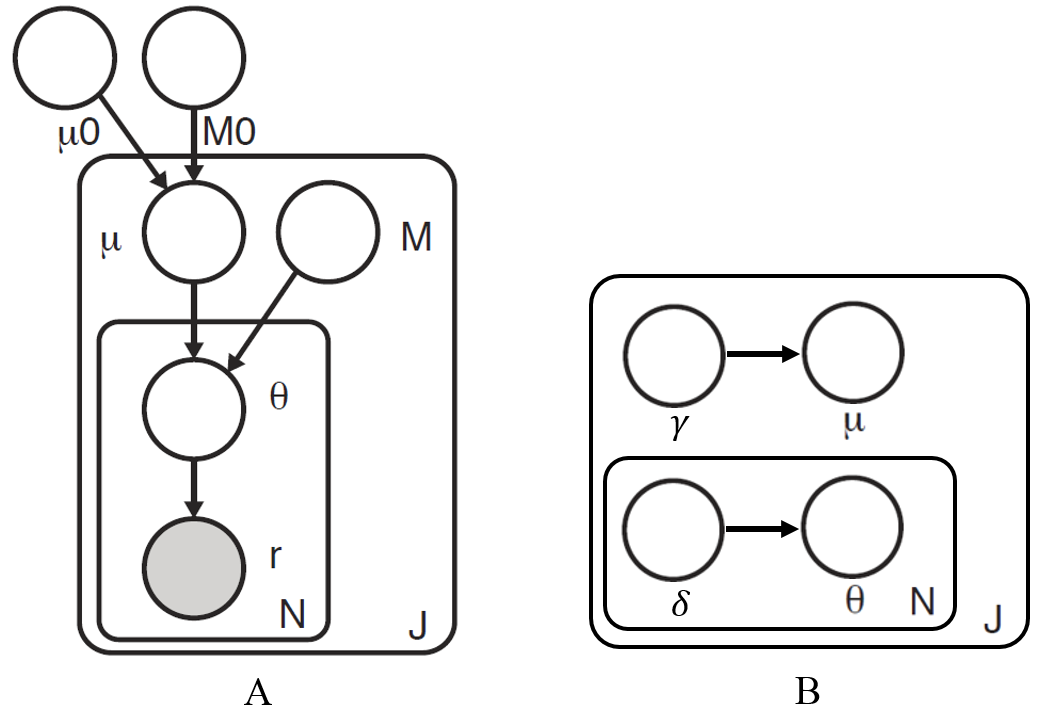
\includegraphics[width=0.5\textwidth]{figs/rvd3_model.png}
\caption{A. Graphical model representation of the model.
B. Graphical model representation of the variational approximation  to approximate the posterior distribution.
Observed random variables are shown as shaded nodes and latent random variables are unshaded.
The object of inference for the variational EM algorithm is the joint distribution $p(\mu, \theta|r, n)$.}
\label{tbl:graphical_model}
\end{figure}
The model generative process is as follows:
\begin{enumerate}[noitemsep]
    \item For each location $j \in [1, \ldots, J]$:
	\begin{enumerate}
		\item Draw an error rate $\mu_j \thicksim \text{Beta}(\mu_0, M_0)$
		\item For each replicate $i \in [1, \ldots, N]$:
		\begin{enumerate}
			\item Draw $\theta_{ji} \thicksim \text{Beta}(\mu_j, M_j)$
			\item Draw $r_{ji} | n_{ji} \thicksim \text{Binomial}(\theta_{ji}, n_{ji})$
		\end{enumerate}
	\end{enumerate}
\end{enumerate}


\section{Variational Expectation Maximization (EM) Inference}
%RVD3 improves RVD2 in the way of deterministic posterior distribution inference.
We developed a non-conjugate variational inference algorithm to approximate the posterior distribution,
\begin{equation}
	p(\mu, \theta | r, n; \phi)  = \frac{ p(\mu, \theta, r | n; \phi) } {p ( r | n; \phi)},
\end{equation}
where the parameters are $\phi \triangleq \{\mu_0, M_0, M\}$.
\subsection{Factorization}
We propose the following factorized variational distribution to approximate the true posterior over latent variables $\mu_j$ and $\theta_{ji}$.
Here, $q(\mu_j)$ approximates the variational posterior distribution of $\mu_j$, which represents the local error rate distribution in position $j$ across different replicates;
and $q(\theta_{ji})$ approximates the posterior distribution of $\theta_{ji}$, which is the error rate distribution in position $j$ replicate $i$.
\begin{equation}
  q(\mu, \theta) = q(\mu)q(\theta) = \prod_{j=1}^J q(\mu_{j}) \prod_{i=1}^N q(\theta_{ji}).
  \label{eq:vardist}
\end{equation}
\subsection{Evidence Lower Bound (ELBO)}
Given the variational distribution, $q$, the log-likelihood of the data is lower-bounded according to Jensen's inequality,
\begin{equation}
\begin{split}
\log p \left( r | \phi \right) &= \log \int_\mu \int_\theta p\left(r,\mu,\theta \right) d\theta d\mu \\
&= \log \int_\mu \int_\theta p\left(r,\mu,\theta \right)\frac{q\left(\mu,\theta \right) }{q\left(\mu,\theta \right) } d\theta d\mu \\
&\geq \int_\mu \int_\theta q\left(\mu,\theta \right) \log \frac{ p\left(r,\mu,\theta \right)}{q\left(\mu,\theta \right)} d\theta d\mu \\
&= E_q \left[ \log p\left(r,\mu,\theta \right)\right] - E_q \left[ \log q\left(\mu,\theta \right)\right] \\
&\triangleq \mathcal{L}(q, \phi).
\end{split}
\end{equation}

The function $\mathcal{L}(q, \phi)$ is the evidence of lower bound (ELBO) of the log-likelihood of the data, which is the sum of $q$-expected complete log-likelihood and the entropy of the variational distribution $q$.
The goal of variational inference is to maximize the ELBO.
Equivalently, $q$ is chosen by minimizing the Kullback-Liebler (KL) divergence between the variational distribution and the true posterior distribution.

The ELBO can be expanded as
\begin{equation}
\begin{split}
\label{L}
\mathcal{L}(q, \phi) &= E_q \left[ \log p\left(r,\mu,\theta | n; \phi \right)\right] - E_q \left[ \log q\left(\mu,\theta \right)\right] \\
&= E_q \left[ \log p\left(r | \theta, n \right)\right] + E_q \left[ \log p\left(\theta | \mu; M \right)\right] + E_q \left[ \log p\left(\mu ; \mu_0, M_0 \right)\right]- E_q \left[ \log q\left(\mu \right)\right]- E_q \left[ \log q\left(\theta \right)\right]. \\
\end{split}
\end{equation}
We write out each component below.
The detail of the derivation of $E_q \left[ \log p\left(r | \theta, n \right)\right]$, $E_q \left[ \log p\left(\mu ; \mu_0, M_0 \right)\right]$, and $E_q \left[ \log p\left(\theta | \mu; M \right)\right]$ is shown in Appendix~\ref{appendix:ELBO}.
\begin{equation}
\begin{split}
\label{r}
E_q \left[ \log p\left(r | \theta, n \right)\right] &= \sum_{j=1}^{J} \sum_{i=1}^{N} E_q  \left[ \log p \left( r_{ji} | \theta_{ji}, n_{ji} \right) \right] \\
&= \sum_{j=1}^{J} \sum_{i=1}^{N} \log \left( \frac{ \Gamma(n_{ji}+1) } { \Gamma(r_{ji}+1) \Gamma( n_{ji} - r_{ji} + 1 ) }\right)  \\
&\quad + \sum_{j=1}^{J} \sum_{i=1}^{N} \left\lbrace r_{ji} E_q \left[ \log \theta_{ji} \right] + (n_{ji} - r_{ji}) E_q  \left[  \log (1 - \theta_{ji}) \right] \right\rbrace
\end{split}
\end{equation}
%
\begin{equation}
\begin{split}
\label{mu}
E_q \left[ \log p\left(\mu ; \mu_0, M_0 \right)\right] &= \sum_{j=1}^{J} E_q  \left[ \log p\left( \mu_j; \mu_0, M_0 \right) \right] \\
&= J* \log \frac{ \Gamma(M_0) } { \Gamma(\mu_0 M_0) \Gamma(M_0 (1-\mu_0))} \\
&\quad + \sum_{j=1}^{J} \left\lbrace (M_0\mu_0 -1)E_q  \left[ \log \mu_j \right] + (M_0 ( 1 - \mu_0) - 1) E_q  \left[ \log (1 - \mu_j)\right]\right\rbrace
\end{split}
\end{equation}
%
\begin{equation}
\begin{split}
\label{theta}
E_q \left[ \log p\left(\theta | \mu; M \right)\right] &= \sum_{j=1}^{J} \sum_{i=1}^{N} E_q \left[ \log p\left(\theta_{ji} | \mu_j; M_j \right)\right] \\
&= N* \sum_{j=1}^{J} E_q  \left[ \log \left( \frac{ \Gamma(M_j) } { \Gamma(\mu_j M_j) \Gamma(M_j (1-\mu_j)) }\right) \right] \\
&\quad + \sum_{j=1}^{J} \sum_{i=1}^{N} \left\lbrace M_j E_q \left[ \mu_j \right] E_q \left[ \log \theta_{ji} \right] - E_q  \left[ \log \theta_{ji} \right] + \left( M_j - 1 - M_j E_q\left[ \mu_j \right]  \right) E_q\left[ \log \left( 1 - \theta_{ji}\right) \right] \right\rbrace
\end{split}
\end{equation}
Therefore, we need to compute the following expectations with respect to the variational distribution:
%
$ E_q \left[ \log \theta_{ji} \right] $, $ E_q\left[ \log \left( 1 - \theta_{ji}\right) \right] $ , $ E_q  \left[ \log \mu_j \right] $ , $ E_q  \left[ \log (1 - \mu_j)\right] $, $ E_q \left[ \mu_j \right] $, and $ E_q\left[ \log \left( \frac{ \Gamma(M_j) } { \Gamma(\mu_j M_j) \Gamma(M_j (1-\mu_j)) }\right)\right] $.
We select the functional forms for the variational distributions $q(\theta)$ and $q(\mu)$ to facilitate these expected value computations.

\subsection{Variational Distributions}
Since $\theta$ and $r$ are conjugate pairs, the posterior distribution of $\theta_{ji}$ is a Beta distribution,
\begin{align}
&p(\theta_{ji}|r_{ji},n_{ji},\mu_j,M_j)
\thicksim \text{Beta}(r_{ji}+M_j \mu_j, n_{ji}-r_{ji}+M_j(1-\mu_j)).
\end{align}
Therefore, we propose a Beta distribution with parameter vector $\delta_{ji}$ as variational distribution,
\begin{align}
\theta_{ji} &\thicksim \text{Beta}(\delta_{ji1}, \delta_{ji2}) \nonumber.
\end{align}
%
The posterior distribution of $\mu_j$ is given by its Markov blanket,
\begin{align}
p(\mu_j|\theta_{ji},M_j,\mu_0,M_0)\propto p(\mu_j|\mu_0,M_0)p(\theta_{ji}|\mu_j,M_j).
\end{align}
This is not in the form of any known distribution.
But, since the support of $\mu_j$ is $[0,1]$, we propose Beta distribution with parameter vector $\gamma_{j}$ as a variational distribution,
\begin{align}
\mu_j &\thicksim \text{Beta}(\gamma_{j1}, \gamma_{j2}) \nonumber.
\end{align}
Given these variational distributions, we have
\begin{align}
E_q \left[ \log \theta_{ji} \right] &= \psi(\delta_{ji1}) - \psi(\delta_{ji1}+\delta_{ji2}) \nonumber \\
E_q \left[ \log \left( 1 - \theta_{ji}\right) \right]&= \psi(\delta_{ji2}) - \psi(\delta_{ji1}+\delta_{ji2}) \nonumber \\
E_q \left[ \mu_j \right] &= \frac{\gamma_{j1}}{\gamma_{j1} + \gamma_{j2}} \nonumber \\
E_q  \left[ \log \mu_j \right] &= \psi(\gamma_{j1}) - \psi(\gamma_{j1}+\gamma_{j2}) \nonumber \\
E_q  \left[ \log (1 - \mu_j)\right] &= \psi(\gamma_{j2}) - \psi(\gamma_{j1}+\gamma_{j2})\nonumber. \\
\end{align}
%
Since there is no analytical representation for $ E_q\left[ \log \left( \frac{ \Gamma(M_j) } { \Gamma(\mu_j M_j) \Gamma(M_j (1-\mu_j)) }\right)\right] $, we must resort to numerical integration,

\begin{equation}\label{eqn:integration}
\begin{split}
E_q\left[ \log \left( \frac{ \Gamma(M_j) } { \Gamma(\mu_j M_j) \Gamma((1-\mu_j)M_j ) }\right)\right] &= \int_{0}^{1} q(\mu_j;\gamma_{j1}, \gamma_{j2}) \log \left( \frac{ \Gamma(M_j) } { \Gamma(\mu_j M_j) \Gamma((1-\mu_j)M_j ) }\right) d\mu_j.
%&= \int_{0}^{1}\frac{\mu_j^{\gamma_{j1}-1}(1-\mu_j)^{\gamma_{j2}-1}}{B(\gamma_{j1},\gamma_{j2})}\log \left( \frac{\Gamma (M_j)}{\Gamma (\mu_jM_j)\Gamma ((1-\mu_j)M_j)}\right) d\mu_j\\
%&=\int_{0}^{1}\frac{\mu_j^{\gamma_{j1}-1}(1-\mu_j)^{\gamma_{j2}-1}}{B(\gamma_{j1},\gamma_{j2})}\log \frac{1}{\int_{0}^{1} t^{\mu_jM_j} (1-t)^{(1-\mu_j)M_j} dt} d\mu_j.
\end{split}
\end{equation}
Here $q(\mu_j;\gamma_{j1}, \gamma_{j2})$ is the probability density function of the Beta distribution that is calculated using the Python built-in function \textit{scipy.stats.beta.pdf $ (\mu_j, \gamma_{j1}, \gamma_{j2})$ };
and $\log \left( \frac{ \Gamma(M_j) } { \Gamma(\mu_j M_j) \Gamma((1-\mu_j)M_j ) }\right)$ is calculated using the Python built-in function \textit{scipy.stats.betaln $ (\mu_j M_j, (1-\mu_j)M_j )$ }.
Unfortunately, this numerical integration step is computationally expensive.
%
Finally, the entropy terms can be computed as follows,
\begin{equation}
\begin{split}
E_q \left[ \log q\left(\mu \right)\right] &= \sum_{j=1}^{J} E_q \left[ \log q(\mu_j)\right] \\
&= -\sum_{j=1}^{J} \left\lbrace \log (B(\gamma_{j1},\gamma_{j2})) -(\gamma_{j1}-1)\psi(\gamma_{j1}) \right\rbrace \\
& + \sum_{j=1}^{J} \left\lbrace -(\gamma_{j2}-1)\psi(\gamma_{j2}) + (\gamma_{j1}+\gamma_{j2}-2)\psi(\gamma_{j1}+\gamma_{j2})\right\rbrace;
\end{split}
\end{equation}
and
\begin{equation}
\begin{split}
E_q \left[ \log q\left(\theta \right)\right] &= \sum_{j=1}^{J}\sum_{i=1}^{N} E_q\left[ \log q(\theta_{ji})\right] \\
&= -\sum_{j=1}^{J}\sum_{i=1}^{N} \left\lbrace \log (B(\delta_{ji1},\delta_{ji2}))-(\delta_{ji1}-1)\psi(\delta_{ji1}) \right\rbrace \\
& + \sum_{j=1}^{J}\sum_{i=1}^{N} \left\lbrace -(\delta_{ji2}-1)\psi(\delta_{ji2}) + (\delta_{ji1}+\delta_{ji2}-2)\psi(\delta_{ji1}+\delta_{ji2})\right\rbrace.
\end{split}
\end{equation}
%
\subsection{Variational EM Algorithm}
Variational EM algorithm maximizes the ELBO on the true likelihood by alternating between maximization over $q$ (E-step) and maximization over $\phi= \left\{\mu_0, M_0, M \right\}$ (M-step).
\subsubsection{(E-step): Updating the variational distributions}
The terms in the ELBO that depend on $q(\theta_{ji} | \delta_{ji1}, \delta_{ji2})$ are
\begin{equation}\label{eqn:partial_theta}
\begin{split}
\mathcal{L}_{{[q(\theta_{ji})]}}
& = \sum_{j=1}^{J} \sum_{i=1}^{N} \left\lbrace r_{ji} E_q \left[ \log \theta_{ji} \right] + (n_{ji} - r_{ji}) E_q  \left[  \log (1 - \theta_{ji}) \right] \right\rbrace\\
& +  \sum_{j=1}^{J} \sum_{i=1}^{N} \left\lbrace M_j E_q \left[ \mu_j \right] E_q \left[ \log \theta_{ji} \right] - E_q  \left[ \log \theta_{ji} \right] + \left( M_j - 1 - M_j E_q\left[ \mu_j \right]  \right) E_q\left[ \log \left( 1 - \theta_{ji}\right) \right] \right\rbrace\\
& - \sum_{j=1}^{J}\sum_{i=1}^{N} E_q\left[ \log q(\theta_{ji})\right]
\end{split}
\end{equation}

We update the variational parameters by numerically optimizing $\hat{\delta}_{ij1}, \hat{\delta}_{ij2} = \arg \max_{\delta_{ij1}, \delta_{ij2}} \mathcal{L}_{{[q(\theta_{ji})]}}$ subject to the constraints that $\delta_{ij1} \geq 0$ and $\delta_{ij2} \geq 0$ and conditioned on fixed values for the other model and variational parameters using Sequential Least SQuares Programming (SLSQP) ~\citep{kraft1988software}.

We update the variational distribution $q(\mu_j)$ using the partial ELBO depending on $\gamma_j$ from each position $j$ \eqref{eqn:partial_mu}.
\begin{equation}\label{eqn:partial_mu}
\begin{split}
\mathcal{L}_{{[q(\mu_j)]}}
& = N \sum_{j=1}^{J} E_q  \left[ \log \left( \frac{ \Gamma(M_j) } { \Gamma(\mu_j M_j) \Gamma(M_j (1-\mu_j)) }\right) \right] \\
&\quad + \sum_{j=1}^{J} \sum_{i=1}^{N} \left\lbrace M_j E_q \left[ \mu_j \right] E_q \left[ \log \theta_{ji} \right] - E_q  \left[ \log \theta_{ji} \right] + \left( M_j - 1 - M_j E_q\left[ \mu_j \right]  \right) E_q\left[ \log \left( 1 - \theta_{ji}\right) \right] \right\rbrace\\
& + J \log \frac{ \Gamma(M_0) } { \Gamma(\mu_0 M_0) \Gamma(M_0 (1-\mu_0))} \\
&\quad + \sum_{j=1}^{J} \left\lbrace (M_0\mu_0 -1)E_q  \left[ \log \mu_j \right] + (M_0 ( 1 - \mu_0) - 1) E_q  \left[ \log (1 - \mu_j)\right]\right\rbrace\\
& - \sum_{j=1}^{J} E_q \left[ \log q(\mu_j)\right]
\end{split}
\end{equation}
Again, we update the variational parameters by numerically optimizing $\hat{\gamma}_{j1}, \hat{\gamma}_{j2} = \arg \max_{\gamma_{j1}, \gamma_{j2}} \mathcal{L}_{{[q(\mu_{i})]}}$ subject to the constraints that $\gamma_{j1} \geq 0$ and $\gamma_{j2} \geq 0$ and conditioned on fixed values for the other model and variational parameters using Sequential Least SQuares Programming (SLSQP) ~\citep{kraft1988software}.
The computational cost of optimizing \ref{eqn:partial_mu} is high because of the quadrature integration of $E_q\left[ \log \left( \frac{ \Gamma(M_j) } { \Gamma(\mu_j M_j) \Gamma(M_j (1-\mu_j)) }\right)\right]$ in \eqref{eqn:integration}.


\subsubsection{(M-step): Updating the model parameters}
We can write out the ELBO as a function of each model parameter $\mu_0$, $M_0$, and $M_j$ as follows.

% Optimizing mu0
The ELBO with respect to $ \mu_0 $ is
\begin{equation}\label{eqn:mu_0}
\begin{split}
\mathcal{L}_{[\mu_0]}
&= -J*\log  \Gamma(\mu_0 M_0) - J*\log \Gamma(M_0 (1-\mu_0))
+ M_0\mu_0\sum_{j=1}^{J} \left\lbrace E_q  \left[ \log \mu_j \right]
- E_q  \left[ \log (1 - \mu_j)\right]\right\rbrace . \\
\end{split}
\end{equation}


% Optimizing M0
The ELBO with respect to $ M_0 $ is
\begin{equation}\label{eqn:M_0}
\begin{split}
\mathcal{L}_{[M_0]}
&=J* \log \frac{ \Gamma(M_0) } { \Gamma(\mu_0 M_0) \Gamma(M_0 (1-\mu_0))}
+ M_0 \sum_{j=1}^{J} \left\lbrace \mu_0E_q  \left[ \log \mu_j \right] + ( 1 - \mu_0) E_q  \left[ \log (1 - \mu_j)\right]\right\rbrace.  \\
\end{split}
\end{equation}


% Optimizing M
The ELBO with respect to $M_j$ is
\begin{equation}\label{eqn:M}
\begin{split}
\mathcal{L}_{{[M_j]}}
&= N* \sum_{j=1}^{J} E_q  \left[ \log \left( \frac{ \Gamma(M_j) } { \Gamma(\mu_j M_j) \Gamma(M_j (1-\mu_j)) }\right) \right] \\
&\quad + M_j \sum_{j=1}^{J} \sum_{i=1}^{N} \left\lbrace E_q \left[ \mu_j \right] E_q \left[ \log \theta_{ji} \right] + \left( 1 - E_q\left[ \mu_j \right]  \right) E_q\left[ \log \left( 1 - \theta_{ji}\right) \right] \right\rbrace. \\
\end{split}
\end{equation}
We also use SLSQP to optimize the ELBO function with respect to each parameter, $\mu_0$, $M_0$, and $M$.
It is computationally easy to optimize $\mu_0$ \eqref{eqn:mu_0} and $M_0$ \eqref{eqn:M_0}.
However, it is costly for optimizing $M$ \eqref{eqn:M} because the quadrature numerical integration is needed for calculation of $ E_q\left[ \log \left( \frac{ \Gamma(M_j) } { \Gamma(\mu_j M_j) \Gamma(M_j (1-\mu_j)) }\right)\right] $ using \eqref{eqn:integration}.

The variational EM algorithm is summarized using pseudocode in Algorithm 1.
\begin{algorithm}[ht]
  \caption{Variational EM Inference}

  \begin{algorithmic}[1]

  \State Initialize $q(\theta, \mu)$ and $\hat{\phi}$

  \Repeat

	\Repeat

		\For {j = 1 to J}
			\For {i = 1 to N}
			\State Optimize $\mathcal{L}(q, \hat{\phi})$ over $q(\theta_{ji}; \delta_{ji}) = \text{Beta} (\delta_{ji})$
			\EndFor
		\EndFor

        \For {j = 1 to J}
            \State Optimize $\mathcal{L}(q, \hat{\phi})$ over $q(\mu_j; \gamma_j) = \text{Beta} (\gamma_j)$
        \EndFor

    \Until{change in $\mathcal{L}(q,\hat{\phi})$ is small}

    \State Set $\hat{\phi} \leftarrow \arg \max\limits_{\phi}
            \mathcal{L}(\hat{q},\phi)$
  \Until {change in $\mathcal{L}(\hat{q},\phi)$ is small}

  \end{algorithmic}

\end{algorithm}
%
\section{Hypothesis Testing}
%\subsection{Posterior Distribution Test}
% Z-test
The posterior distribution over $\mu_j^{\triangle} \mid r^{case}, r^{control} \triangleq \mu_j|r^{case} - \mu_j|r^{control}$ is the distribution over the change in the non-reference read rate at position $j$ between a case and control sample.
However, we cannot compute the posterior distribution, $\mu_j^{\triangle} | r^{case}, r^{control}$, because we do not have access to the component posterior distributions $\mu_j|r^{case}$ and $\mu_j|r^{case}$.
But, by approximating the distribution of $\mu_j|r^{case}$ and $\mu_j|r^{control}$ as Gaussians with moments matched to the variational posterior distributions, the distribution of $\mu_j^{\triangle} | r^{case}, r^{control}$ can be approximated as a Gaussian.

Under the variational approximation,
\begin{align}
  E_q[\mu_j|r^{case}] &= \frac{\gamma_{j1}^{case}}{\gamma_{j1}^{case} + \gamma_{j2}^{case}}
  \\
  \text{Var}_q[\mu_j|r^{case}] &= \frac{\gamma_{j1}^{case} \gamma_{j2}^{case}}{(\gamma_{j1}^{case} + \gamma_{j2}^{case} + 1)(\gamma_{j1}^{case} + \gamma_{j2}^{case})^2}
\end{align}
for $\mu_j|r^{case}$ and likewise for $\mu_j|r^{control}$.
We approximate the posterior for the case sample as
\begin{equation}
  \mu_j | r^{case} \sim \mathcal{N}(E_q[\mu_j|r^{case}], \text{Var}_q[\mu_j|r^{case}])
\end{equation}
and likewise for the control.
Then,
\begin{equation}
  \mu_j^{\triangle} \mid r^{case}, r^{control} \sim \mathcal{N}(E_q[\mu_j|r^{case}] - E_q[\mu_j|r^{control}], \text{Var}_q[\mu_j|r^{case}] + \text{Var}_q[\mu_j|r^{control}])
\end{equation}

Now, we can approximate the posterior probability of interest,
\begin{equation}
  \Pr( \mu_j^{\triangle} \geq \tau \mid r^{case}, r^{control} ),
\end{equation}
that is, the posterior probability that the difference in the non-reference read rate is greater than a fixed effect size $\tau$ (e.g. zero) for a one sided test.
For a two sided test, we compute the approximate probability
\begin{equation}
  \Pr( | \mu_j^{\triangle} | \geq \tau \mid r^{case}, r^{control}).
\end{equation}
A position is called a \textit{provisional variant} if $\Pr( | \mu_j^{\triangle} | \geq \tau \mid r^{case}, r^{control}) \geq 1-\alpha/2$, where the probability is approximated as described.

% Chi-square test
It is possible that a position is called a variant due to a differential non-reference read count, but no particular alternative base is more frequently observed than the others.
In this case, the likely case is a sequencing error that indiscriminately incorporates a non-reference base at the position.
To discriminate this non-biological cause from the interesting true variants we use a $\chi^2$ goodness-of-fit test for non-uniform base distribution~\citep{efron2010large, he2015rvd2}.
For each provisional variant, if we reject the null hypothesis that the distribution is uniform, we promote the position to a called variant.


\section{Results}
\subsection{Data Sets}
\subsubsection{Synthetic DNA Sequence Data}
Two random 400bp DNA sequences were synthesized. One sample with 14 loci variants is taken as the case and the other without variants is taken as the control.
Case and control samples were mixed to yield defined NRAF of $0.1\%$, $0.3\%$, $1.0\%$, $10.0\%$, and $100.0\%$.
The details of the experimental protocol are available in ~\citep{flaherty2011ultrasensitive}.
The synthetic DNA data were downsampled by 10$\times$, 100$\times$, 1,000$\times$, and 10,000$\times$ using Picard.
The final data set contains read pairs for 6 replicates for the control and cases at different NRAF levels.
\subsubsection{Longitudinal Directed Evolution Data}
The longitudinal yeast data comes from three strains of haploid S288c which were grown for 448 generations under limited-glucose (0.08$\%$).
The Illumina sequencing data are available on NCBI with number SRA054922.
The wild-type ancestral strain GSY1136 was sequenced as a reference.
Aliquots were taken about every 70 generations and sequenced.
The detail of library sequencing is described in ~\citep{kvitek2013whole, kao2008molecular}.
The aligned BAM files have 266-1046$\times$ coverage.
We used SAMtools -mpileup to convert BAM files to pileup files.
Then we generated depth chart files, which are tab-delimited text files recording the count of the number of nucleotides in columns and genomic positions in rows.
We ran our variational inference algorithm on the depth chart files to identify SNVs.
\subsection{Performance on Synthetic DNA Data}
\subsubsection{Comparison of Sensitivity and Specificity}
We compared the performance of our variational EM algorithm and the MCMC sampling algorithm in the performance of sensitivity and specificity (Table~\ref{tbl:statistics_mcmc_var}).
We used the posterior distribution test and $\chi^2$ test to detect variants for a broad range of median read depths and different NRAFs.
The variational EM algorithm works better than the MCMC algorithm in sensitivity and specificity in the events when NRAF is 0.1\%.
The variational EM algorithm has higher specificity compared with the MCMC algorithm in the events of 41472$\times$ at 0.3\% NRAF and 55489 $\times$ at 1.0\% NRAF with a slight degradation in sensitivity due to false negatives.
% results are under folder \fzhang\Research\rvd3-variational-notebook\results\2015-09-28_Run_rvd3_synthetic_data_set
\begin{table}[ht]
\centering
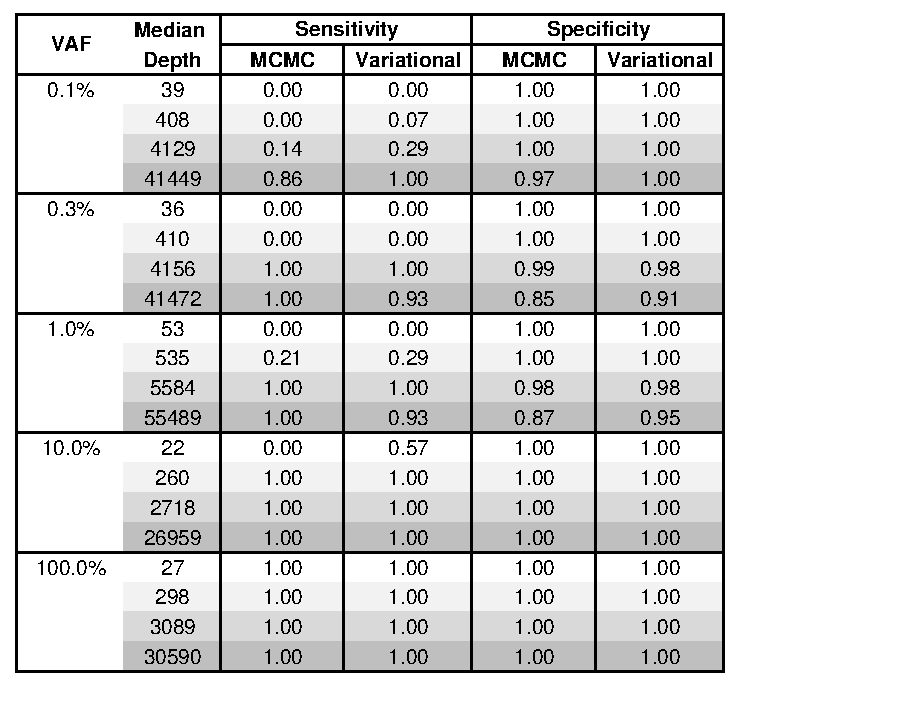
\includegraphics[width=0.8\textwidth]{tables/statistics_mcmc_var.pdf}
\caption{Sensitivity/Specificity comparison of variational EM algorithm with the MCMC algorithm on the synthetic DNA data set.}
\label{tbl:statistics_mcmc_var}
\end{table}
\subsubsection{Comparison of Approximated Posterior Distribution}
We showed the approximated posterior distribution of the variational EM algorithm and exact samples of the MCMC algorithm.
One variant position 85 is taken as an example to show the comparison of the approximated posteriors (Figure~\ref{tbl:compare1}).
The variational and MCMC algorithms both identify all the variants when NRAF is 10.0\% and 100.0\%.
The variational EM algorithm calls some false positive positions without a $\chi^2$ test when NRAFs are 0.1\% and 0.3\% for low median read depth (30$\times$ and 400$\times$).
Here, a non-mutated position that is called by the variational algorithm while not called by the MCMC algorithm is shown in Figure~\ref{tbl:compare2}.
The variance of MCMC posterior distribution is wider than that of the variational algorithm.
To increase the specificity of our variational EM algorithm, the $\chi^2$ test is used to filter this false positive position with an uniform base distribution over the non-reference bases.
We tested 10 random initial values for the posterior distributions and the approximated posterior distributions by the variational EM algorithm are the same.
It is noticeable that the shape of the proposed Beta variational distribution is exactly displayed as a Gaussian distribution.
% results are under folder \fzhang\Research\rvd3-variational-notebook\results\2015-10-14_Plot_mcmc_mu_vs_variational_mu
\begin{figure}[htbp]
\centering
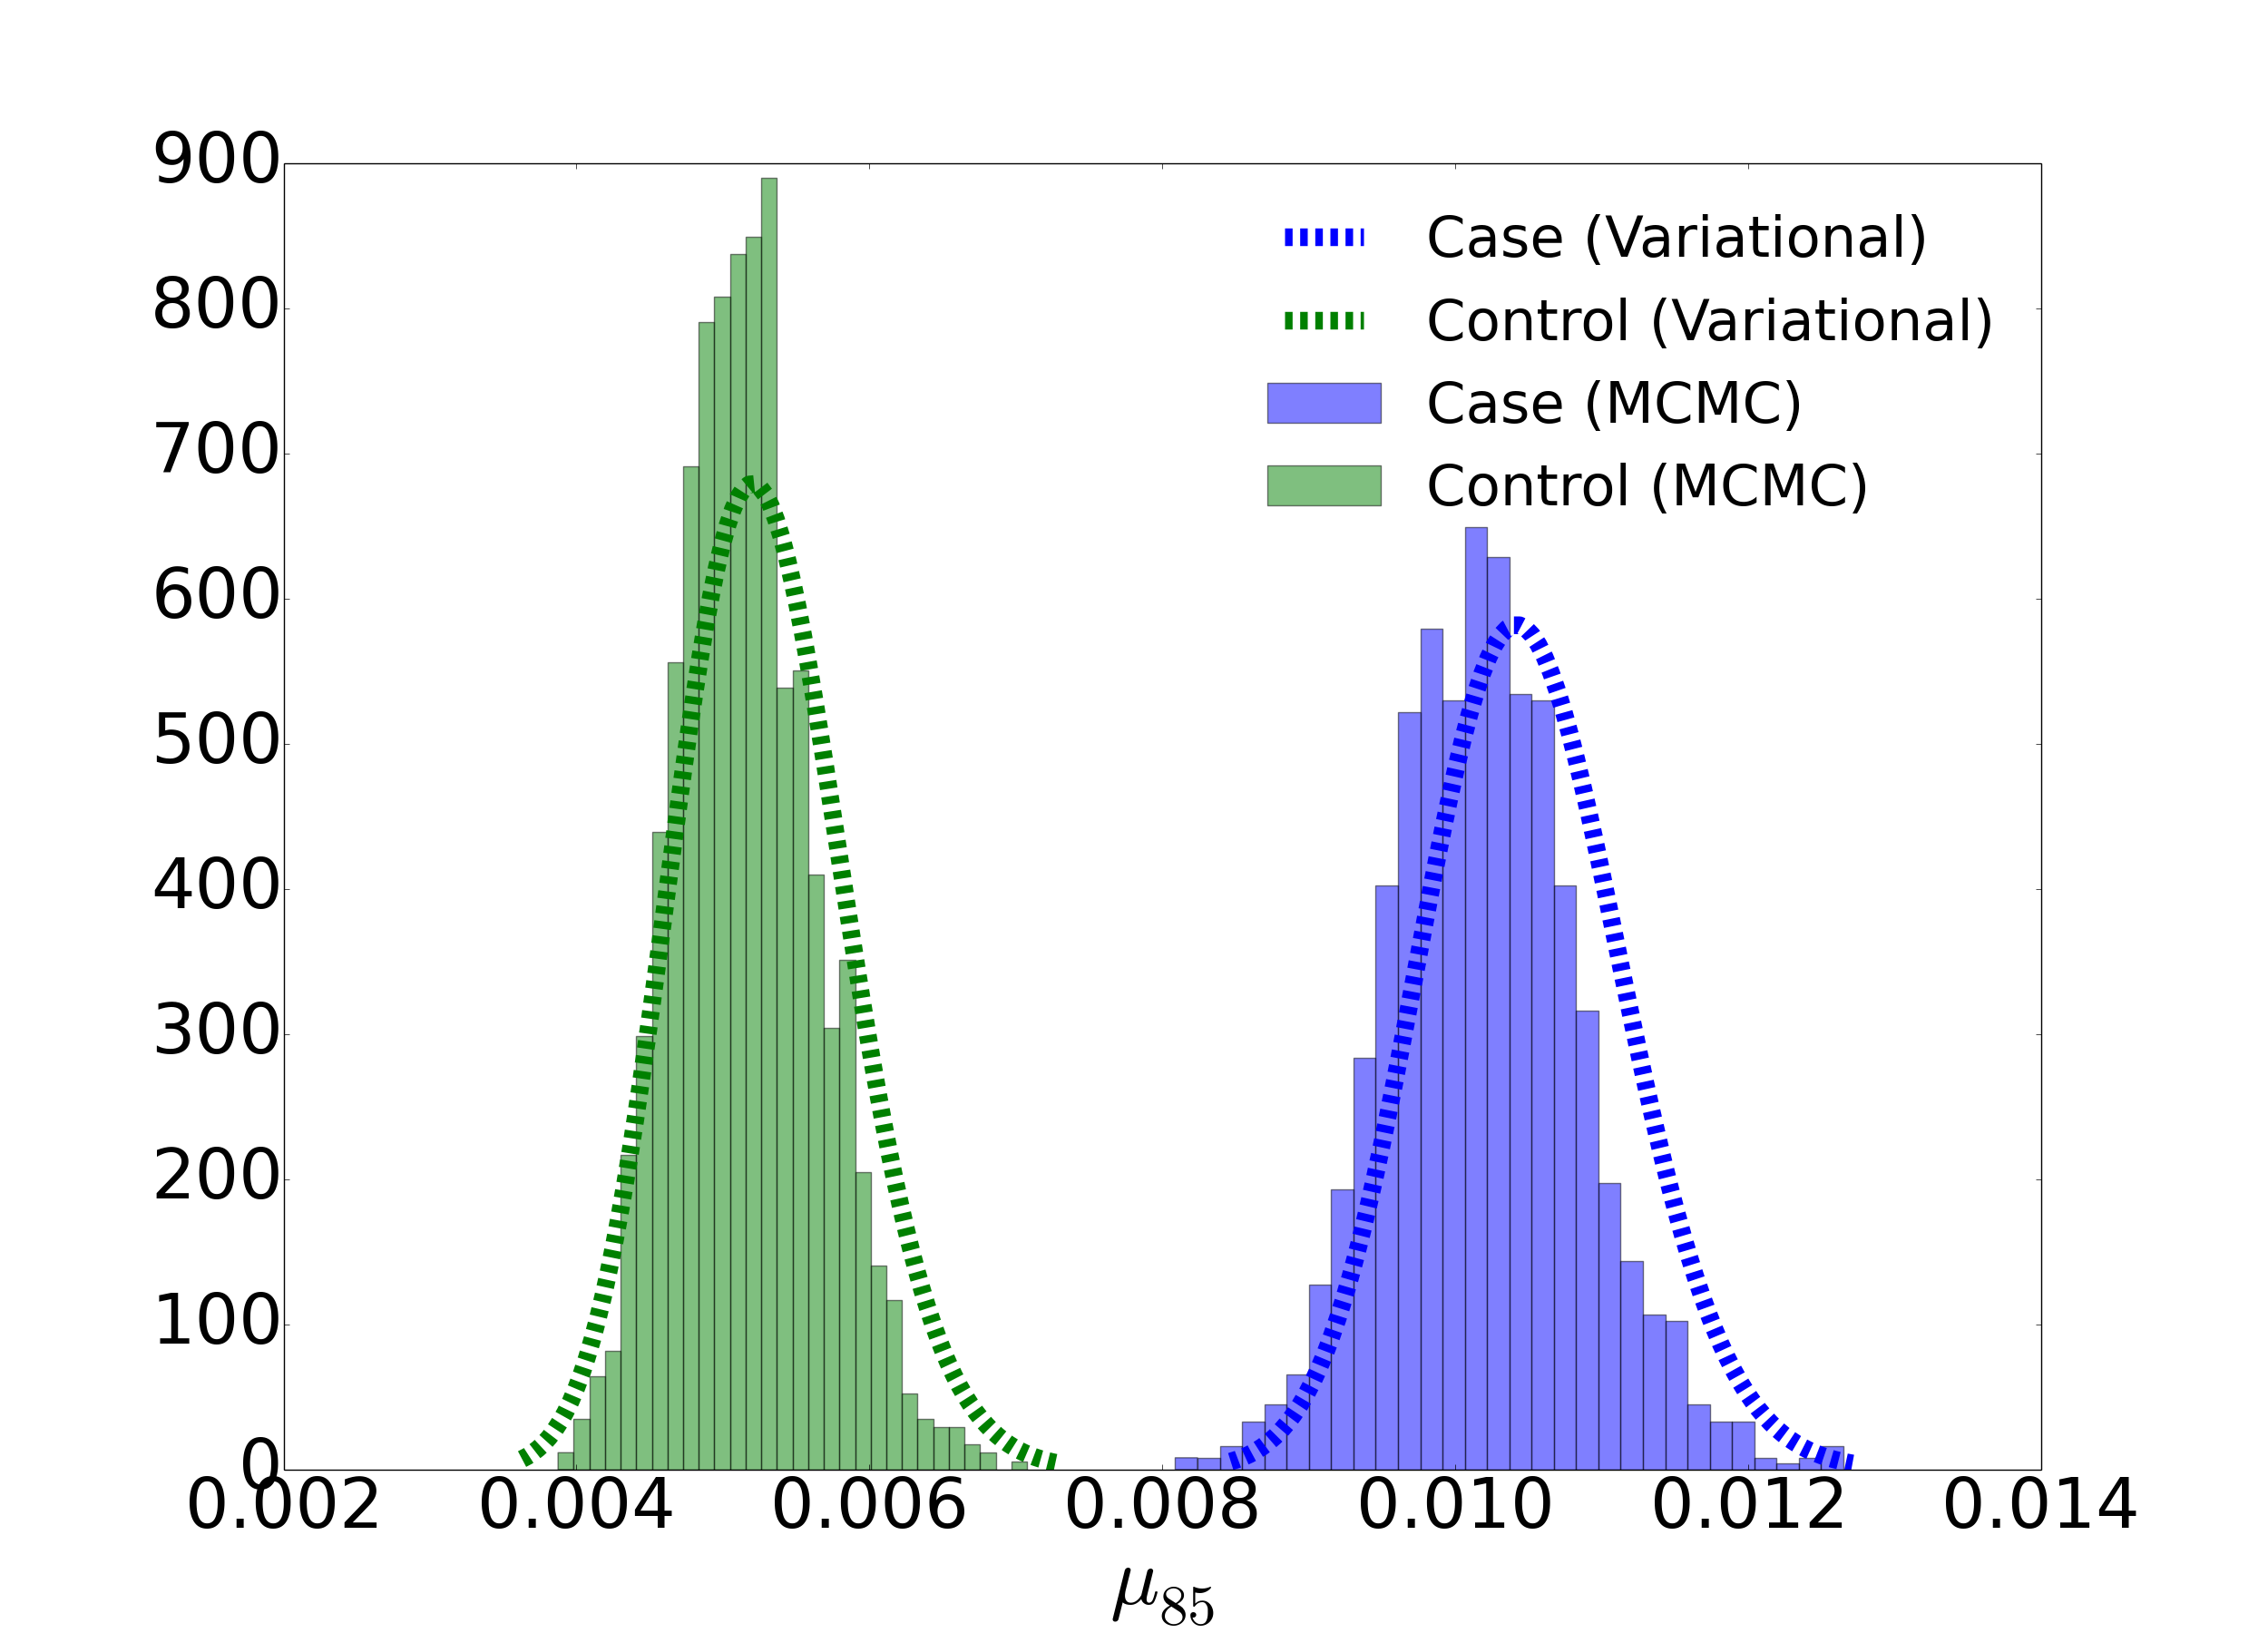
\includegraphics[width=0.7\textwidth]{figs/position_85_5584_mcmc_vs_var_mu_fig1.png}
\caption{Approximated posterior distributions by the variational EM and MCMC algorithms on a true variant position 85 when the median read depth is 5584$\times$.}
\label{tbl:compare1}
\end{figure}
\begin{figure}[htbp]
\centering
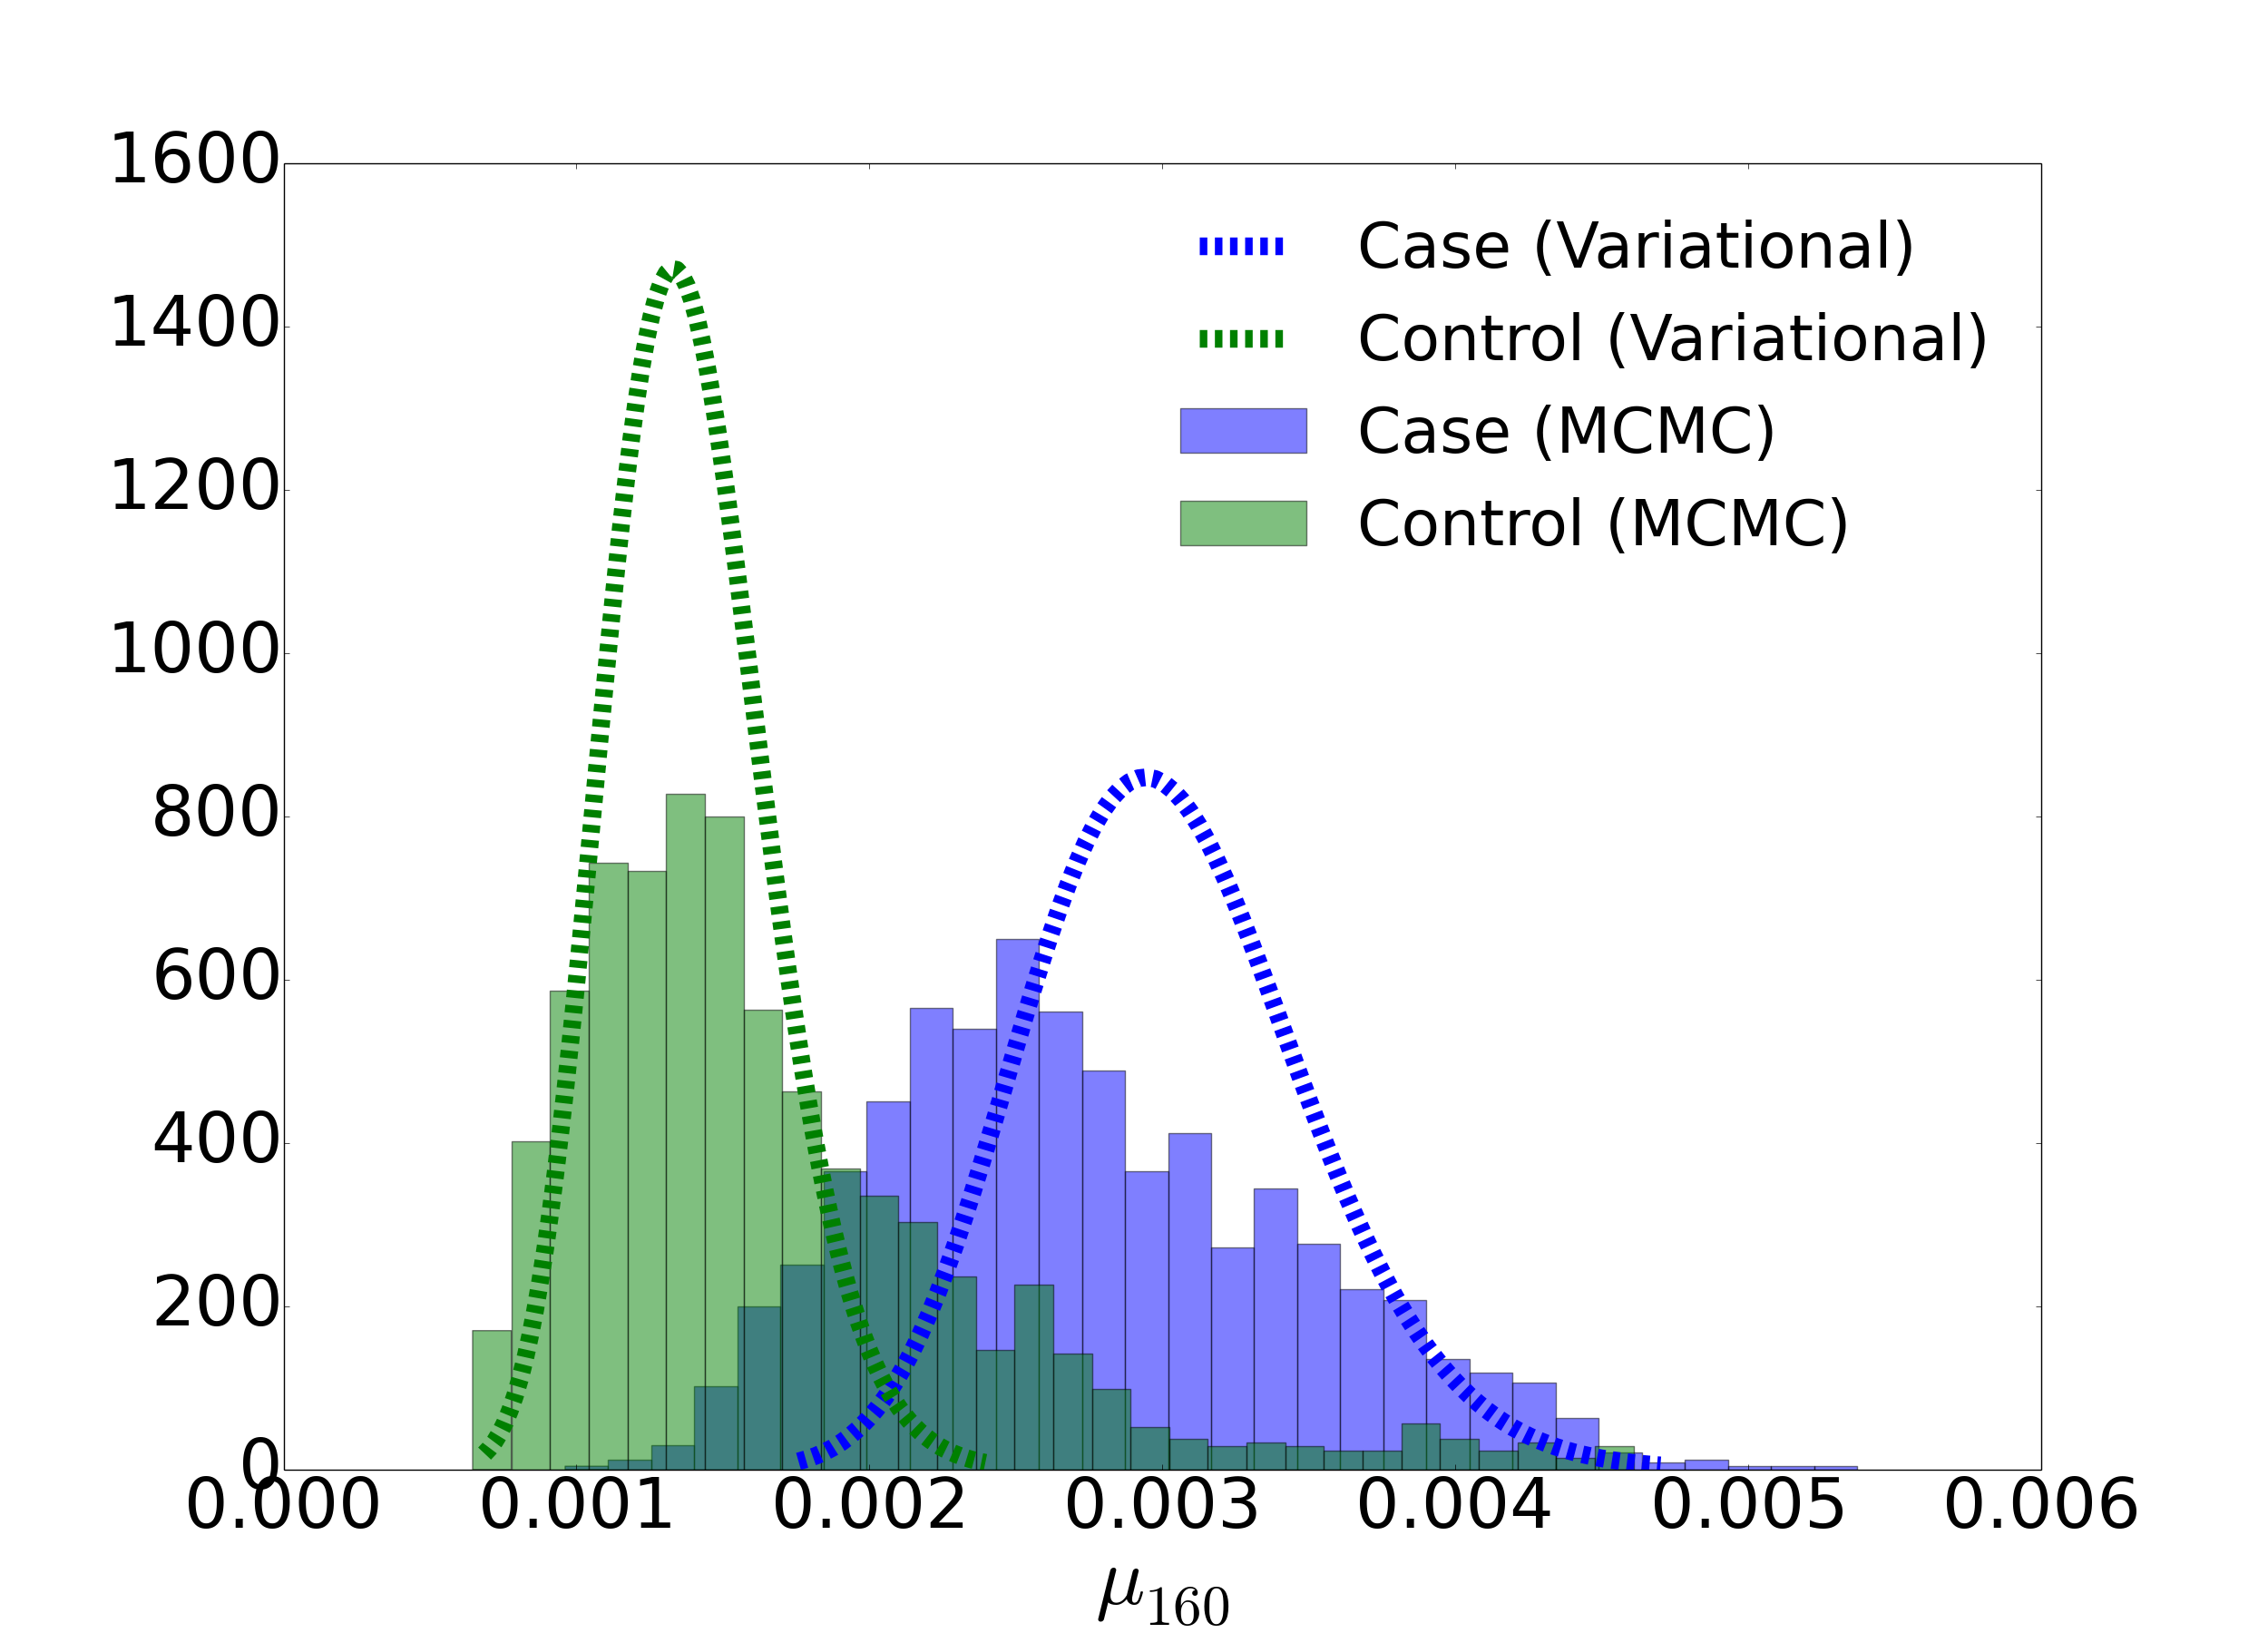
\includegraphics[width=0.7\textwidth]{figs/position_160_410_mcmc_vs_var_mu_fig2.png}
\caption{Approximated posterior distribution by the variational EM and MCMC algorithms on a false variant position 160 when the median read depth is 410$\times$.}
\label{tbl:compare2}
\end{figure}
\subsubsection{Comparison to the State-of-the-Art Methods}
We compared the performance of our variational EM inference algorithm with the state-of-the-art variant detection methods using synthetic DNA data set (Table~\ref{tbl:character_all}).
Among all of the methods compared, our variational inference algorithm shows a high sensitivity and specificity for a broad range of read depths and NRAFs.
Variational inference algorithm also performs higher specificity than all the other tested methods at a very low NRAF (0.1\%) level.
Variational inference algorithm has a slightly lower specificity than the MCMC algorithm only when the median read depth is 4156$\times$ at 0.3\% NRAF, and a slightly lower sensitivity than the MCMC algorithm only when the median read depth is 41472$\times$ at 0.3\% NRAF and a median read depth of 55489$\times$ at 1.0\% NRAF.
The performance of other methods is stated in detail in ~\citep{he2015rvd2}.
\begin{table*}[htbp]
\centering
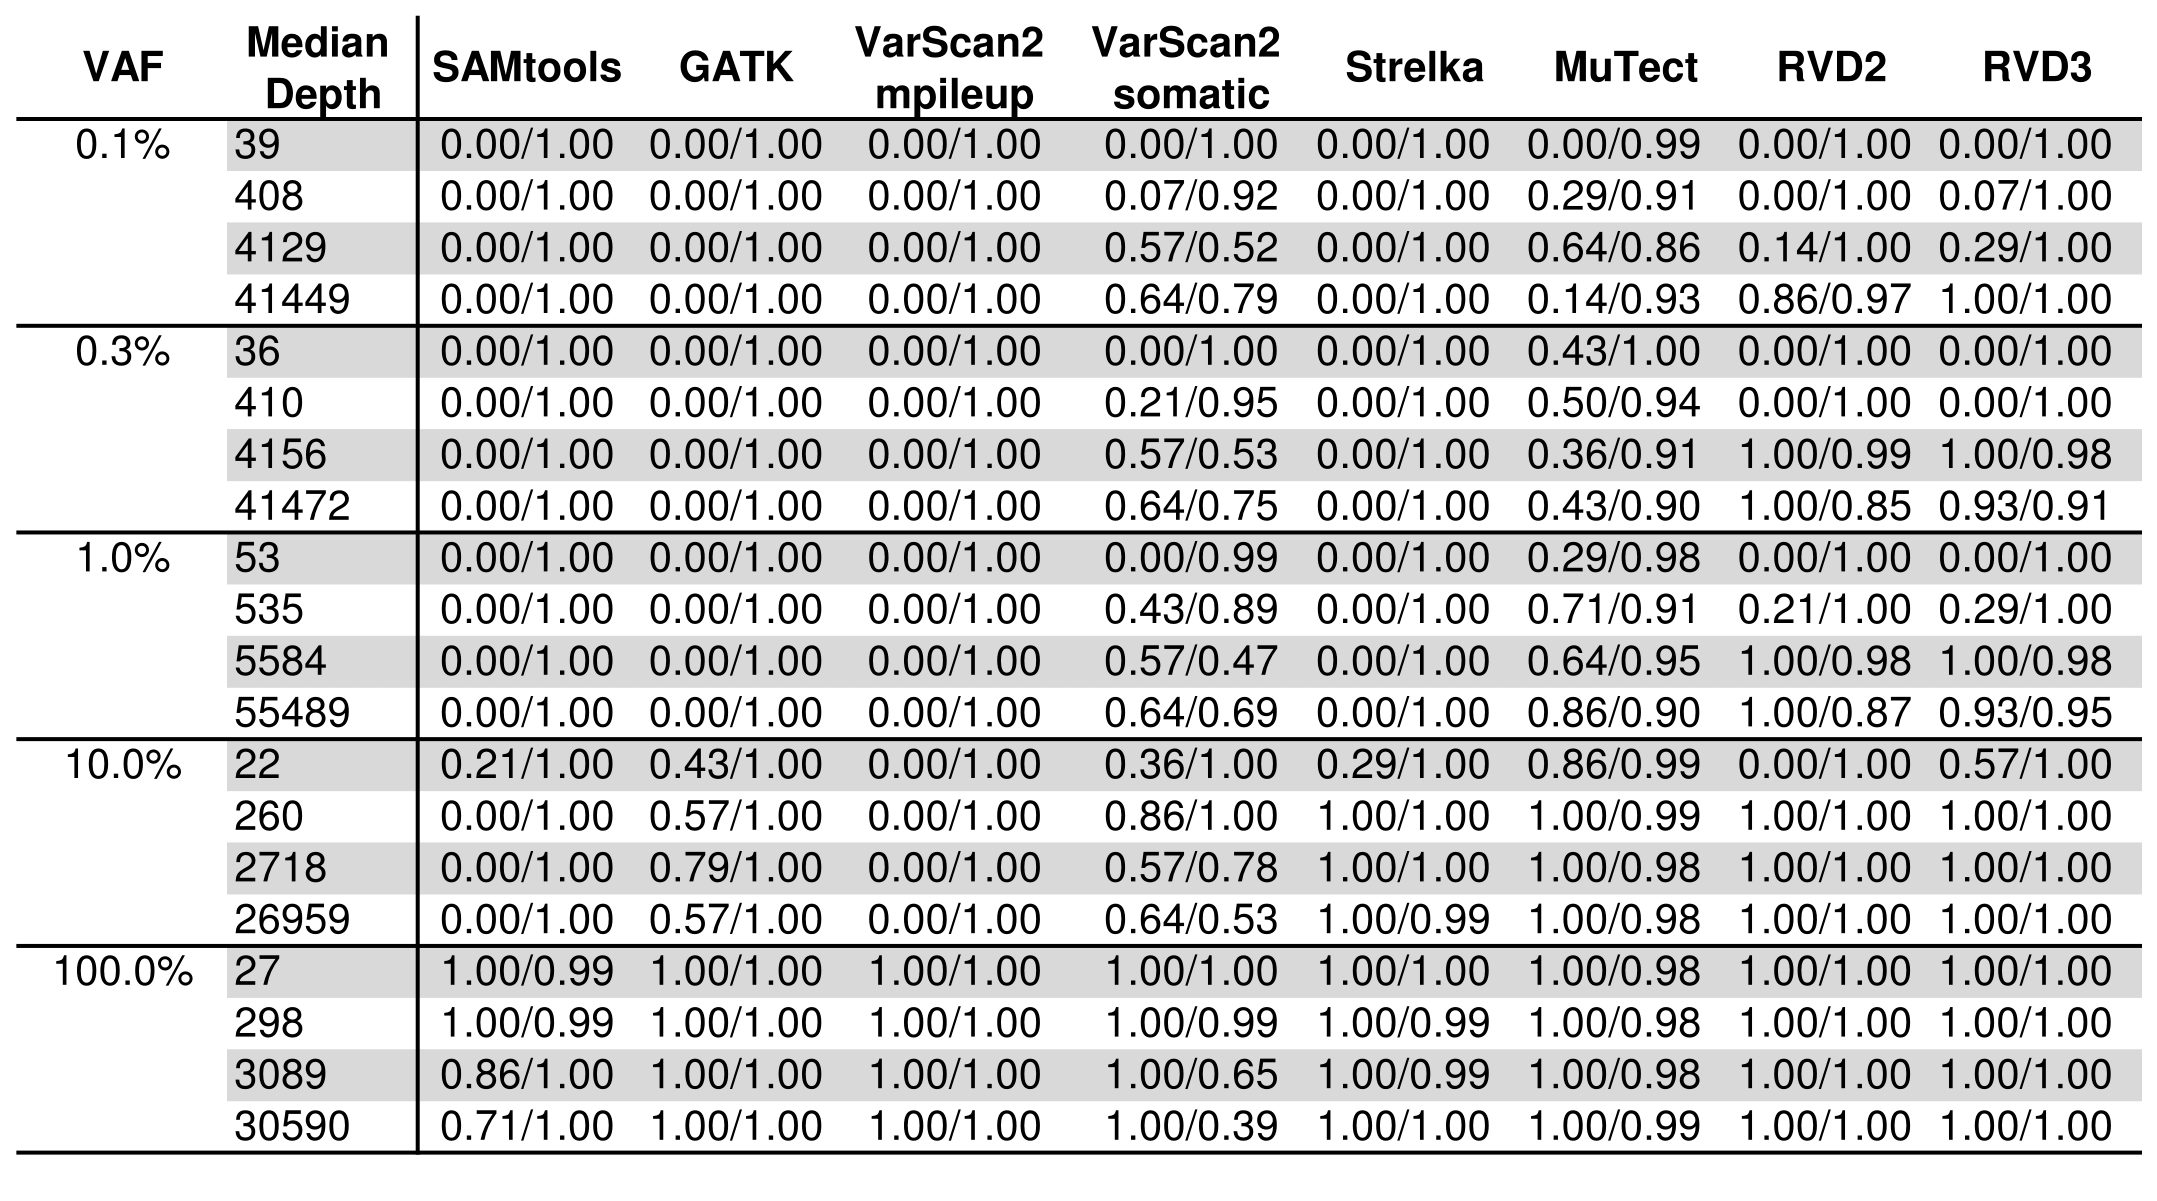
\includegraphics[width=1.0\textwidth]{tables/character_all.png}
\caption{Sensitivity/Specificity comparison of our variational inference algorithm with other variant detection approaches on synthetic DNA data.}
\vspace{-5pt}
\label{tbl:character_all}
\end{table*}
\subsubsection{Comparison of Timing}
% Timing comparison
Time for approximating variational posterior distribution is increased by expanding the length of region and the median read depth (Figure~\ref{tbl:timing_mcmc_var}).
Our variational EM algorithm works faster than the MCMC algorithm at the low median read depths of 27$\times$ and 298$\times$, while it shows the opposite at the high median read depths of 3089$\times$ and 30590$\times$.
% results are under folder \fzhang\Research\rvd3-variational-notebook\results\2015-10-15_Plot_time_vs_region_length_rvd3_synthetic_data
\begin{figure}[ht]
\centering
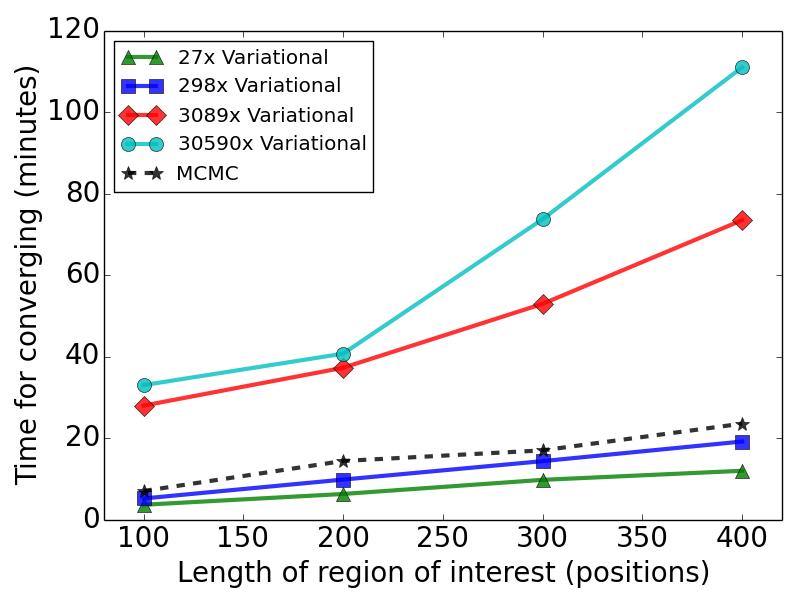
\includegraphics[width=0.6\textwidth]{figs/timing_var_mcmc.png}
\caption{Timing figure for our variational EM algorithm and MCMC sampling algorithm.
Parallel computational cores (60 processers) are used to estimate the model on the synthetic data set.}
\label{tbl:timing_mcmc_var}
\end{figure}
% Timing profile of variational
Furthermore, we show the timing profile for each part of our variational EM algorithm when median read depth is 3089$\times$ (Table~\ref{tbl:timing_profile_all}).
Optimizing $\gamma$ function \eqref{eqn:partial_mu} in E-step and optimizing $M$ \eqref{eqn:M} in M-step take more than 95\% of the time of one variational iteration in a test of a single processor, as such a time consuming integration \eqref{eqn:integration} is needed.
% results are under folder \fzhang\Research\rvd3-variational-notebook\results\2015-10-21_Timing_profile_rvd3_program
\begin{table*}[htbp]
\centering
\vspace{10pt}
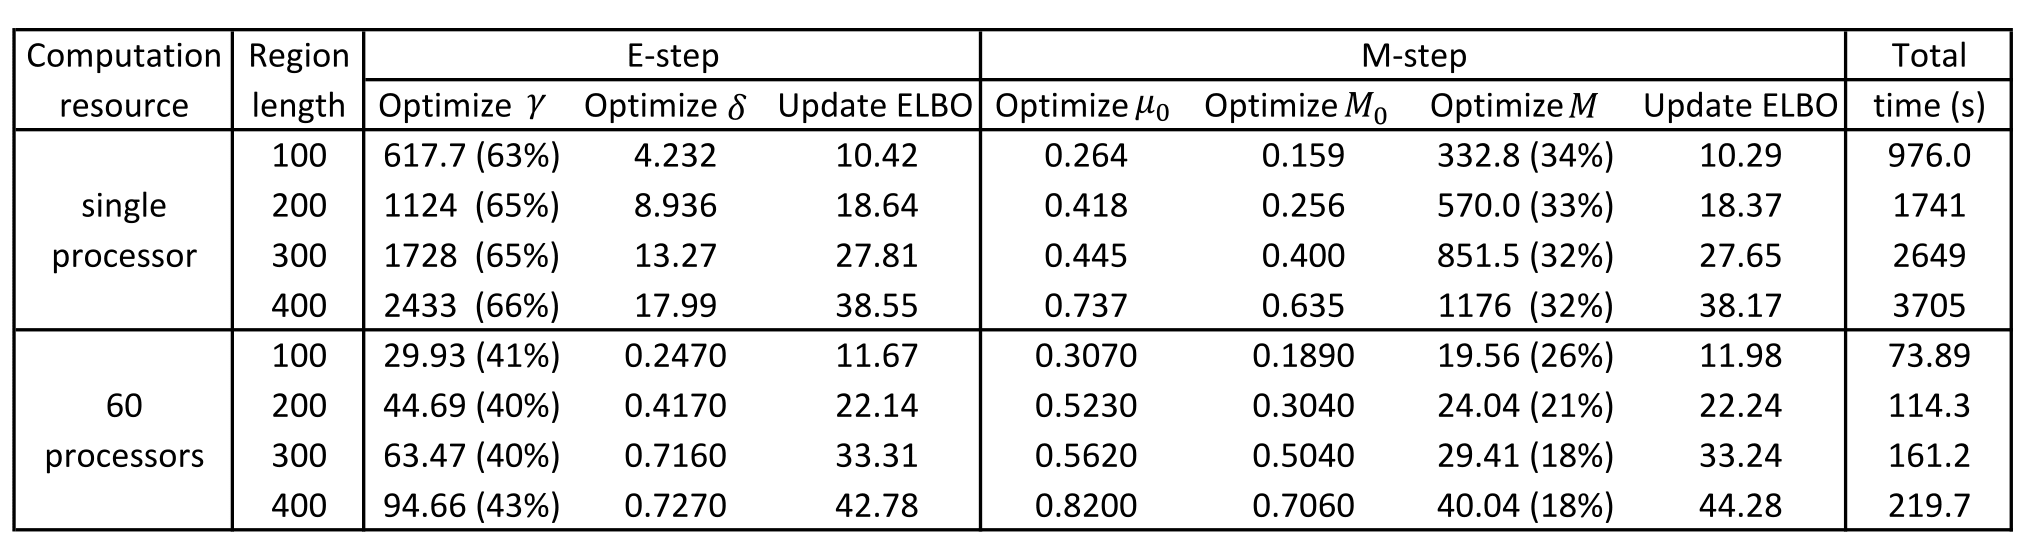
\includegraphics[width=1.0\textwidth]{tables/time_3089X_all_update.png}
\caption{Timing profile of 4 significant figures for one iteration of variational EM algorithm when median read depth is 3089$\times$.
Single and multiple processors are both tested to estimate timing. Time for optimizing $\gamma$ function in E-step and optimizing $M$ in M-step is highlighted in percentage.}
\label{tbl:timing_profile_all}
\end{table*}
\subsection{Variant Detection on the Longitudinal Directed Evolution Data}
% Generally describe detected variants
We applied our variational inference algorithm on the MTH1 gene on Chr04:1014401-1015702, region of 1302bp, which is the most frequently observed mutated gene ~\citep{kvitek2013whole}.
Our variational algorithm detected the same variants that were found by Kvitek and Sherlock, 2013 and marked as blue in Table~\ref{tbl:mutations}.
Additionally, we detected 81 novel variants in 8 timepoints that the original publication missed.
In Table~\ref{tbl:mutations}, G7 is the baseline NRAF as the control sample when comparing with G70, G133, G266, G322, G385, and G448 in the respective hypotheses testing.
The corresponding NRAFs of called variants in different time points are given by the estimation of the latent variable $\mu_j$.
% results are under folder \fzhang\Research\rvd3-variational-notebook\results\2016-01-12_Run_rvd3_Dan_data_regions
\begin{table*}[htbp]
\centering
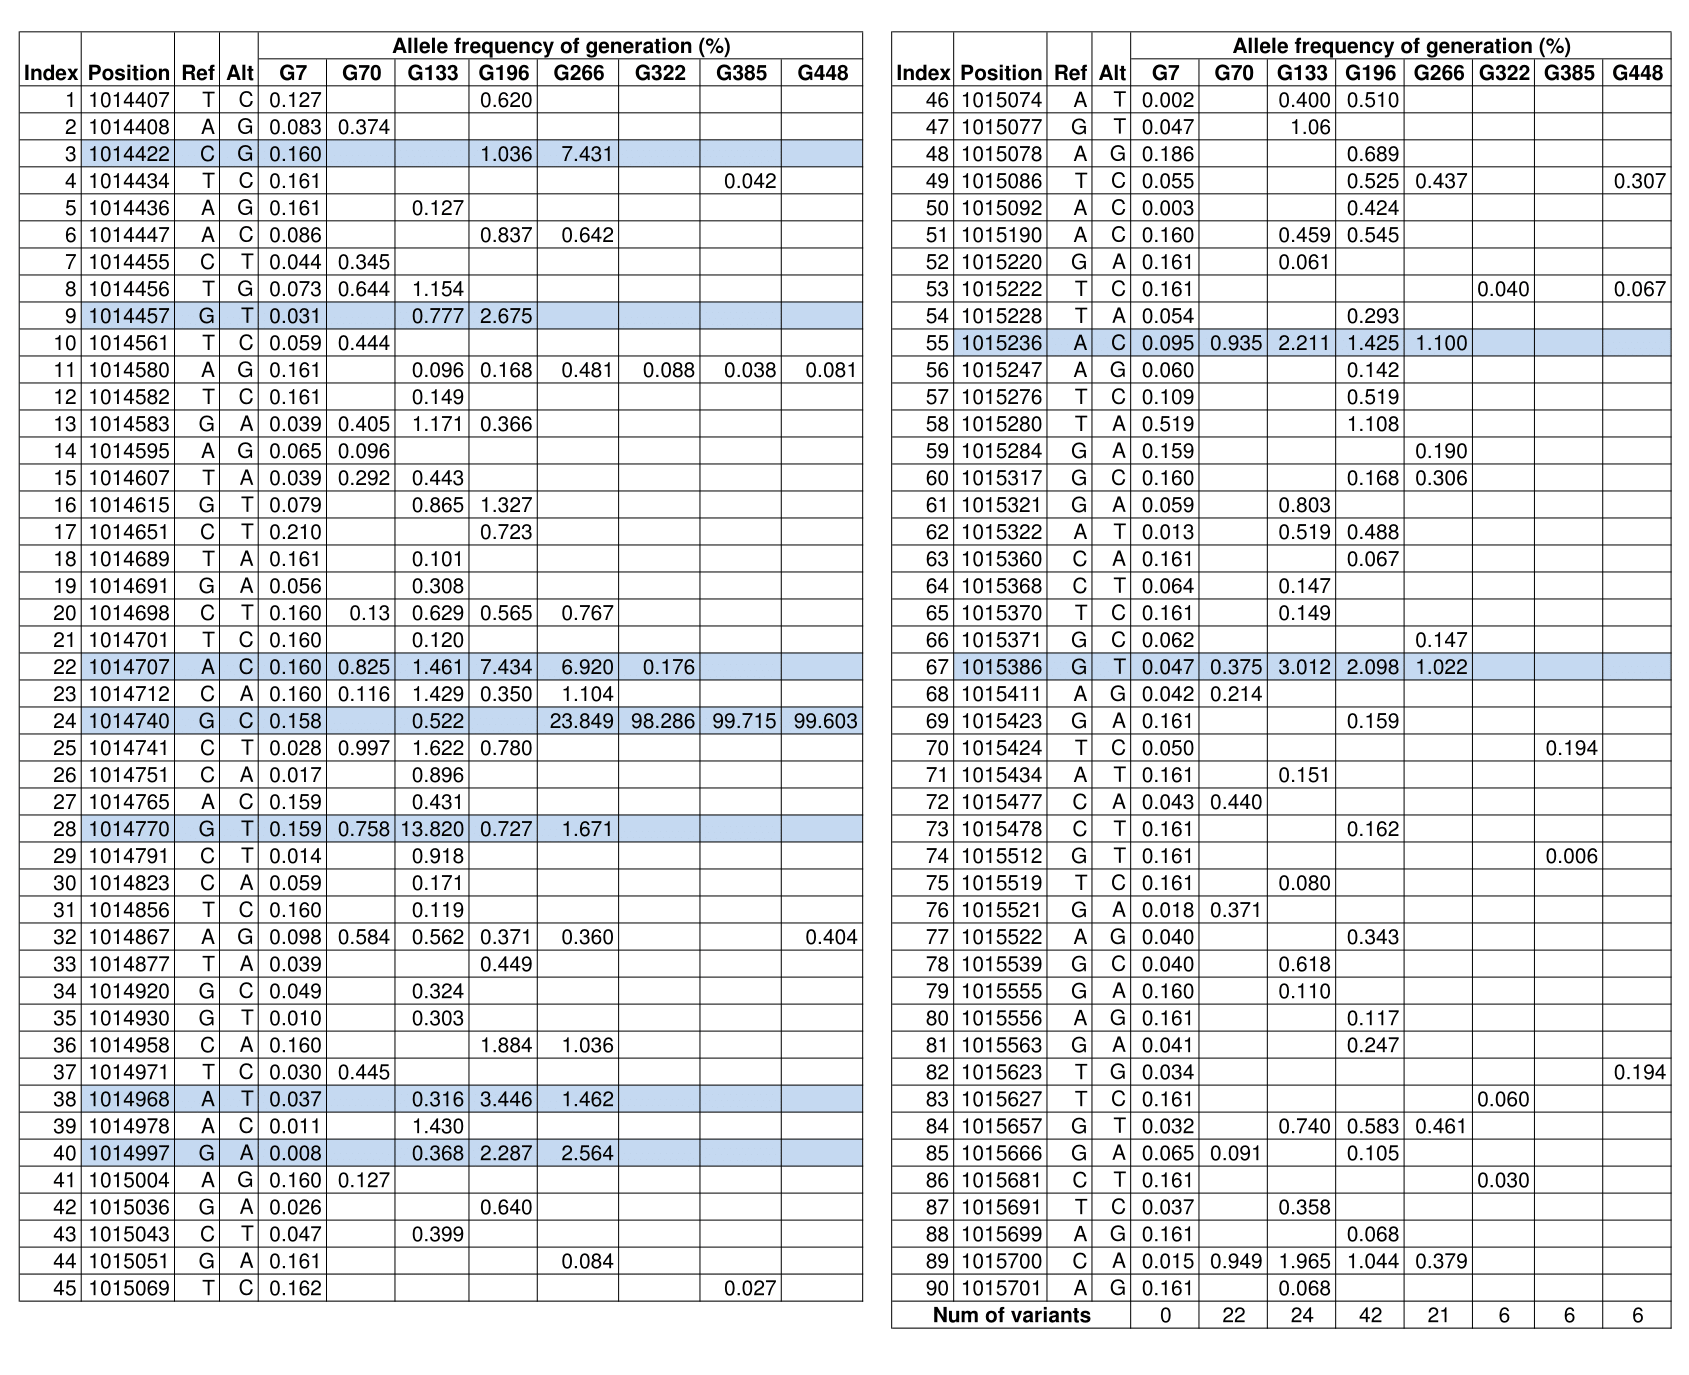
\includegraphics[width=1.0\textwidth]{tables/mutations_MTH1.png}
\caption{Identified variants and corresponding NRAFs in gene MTH1 on Chromosome 4.
A blank cell indicates that the position of that time point is not called significantly different than G7.
Positions marked as blue were also identified by Kvitek, 2013.
Other positions are 81 novel identified variants in 8 timepoints.}
\label{tbl:mutations}
\end{table*}
% Beneficial variant and early identification
All of these variants, except variant in position 1014740, decrease in NRAF following a maximum and eventually become extinct.
Allele on position 1014740 is a beneficial variant that arises in NRAF to 99.603\% at generation 448 within a constant glucose-limited environment.
Moreover, we identified the first emergence of this beneficial variant as early as 0.522\% in generation 133.
Table~\ref{tbl:mutations} shows that we are able to detect many variants (NRAF $<$ 1.0\%) early in the evolutionary time course.
Furthermore, we detected a variant on position 1015666 at generation 70 as 0.091\% NRAF, which is less than a 0.1\% fraction.

% Influence of M0 on muj
As an empirical Bayesian model, the global precision parameter $M_0$ could influence the estimation of $\mu_j$.
We generated a figure to show the influence of different $M_0$ on variant position 1014740 $\mu_{1014740}$.
Figure~\ref{tbl:M0} shows that $\hat{\mu}_{1014740}$ is getting bigger as $M_0$ is getting smaller.
It also reveals that the estimation of $\mu_j$ does not much depend on the changes of $M_0$.
Here $M_0$ equals to 1.752 in this application.
\begin{figure}[htbp]
\centering
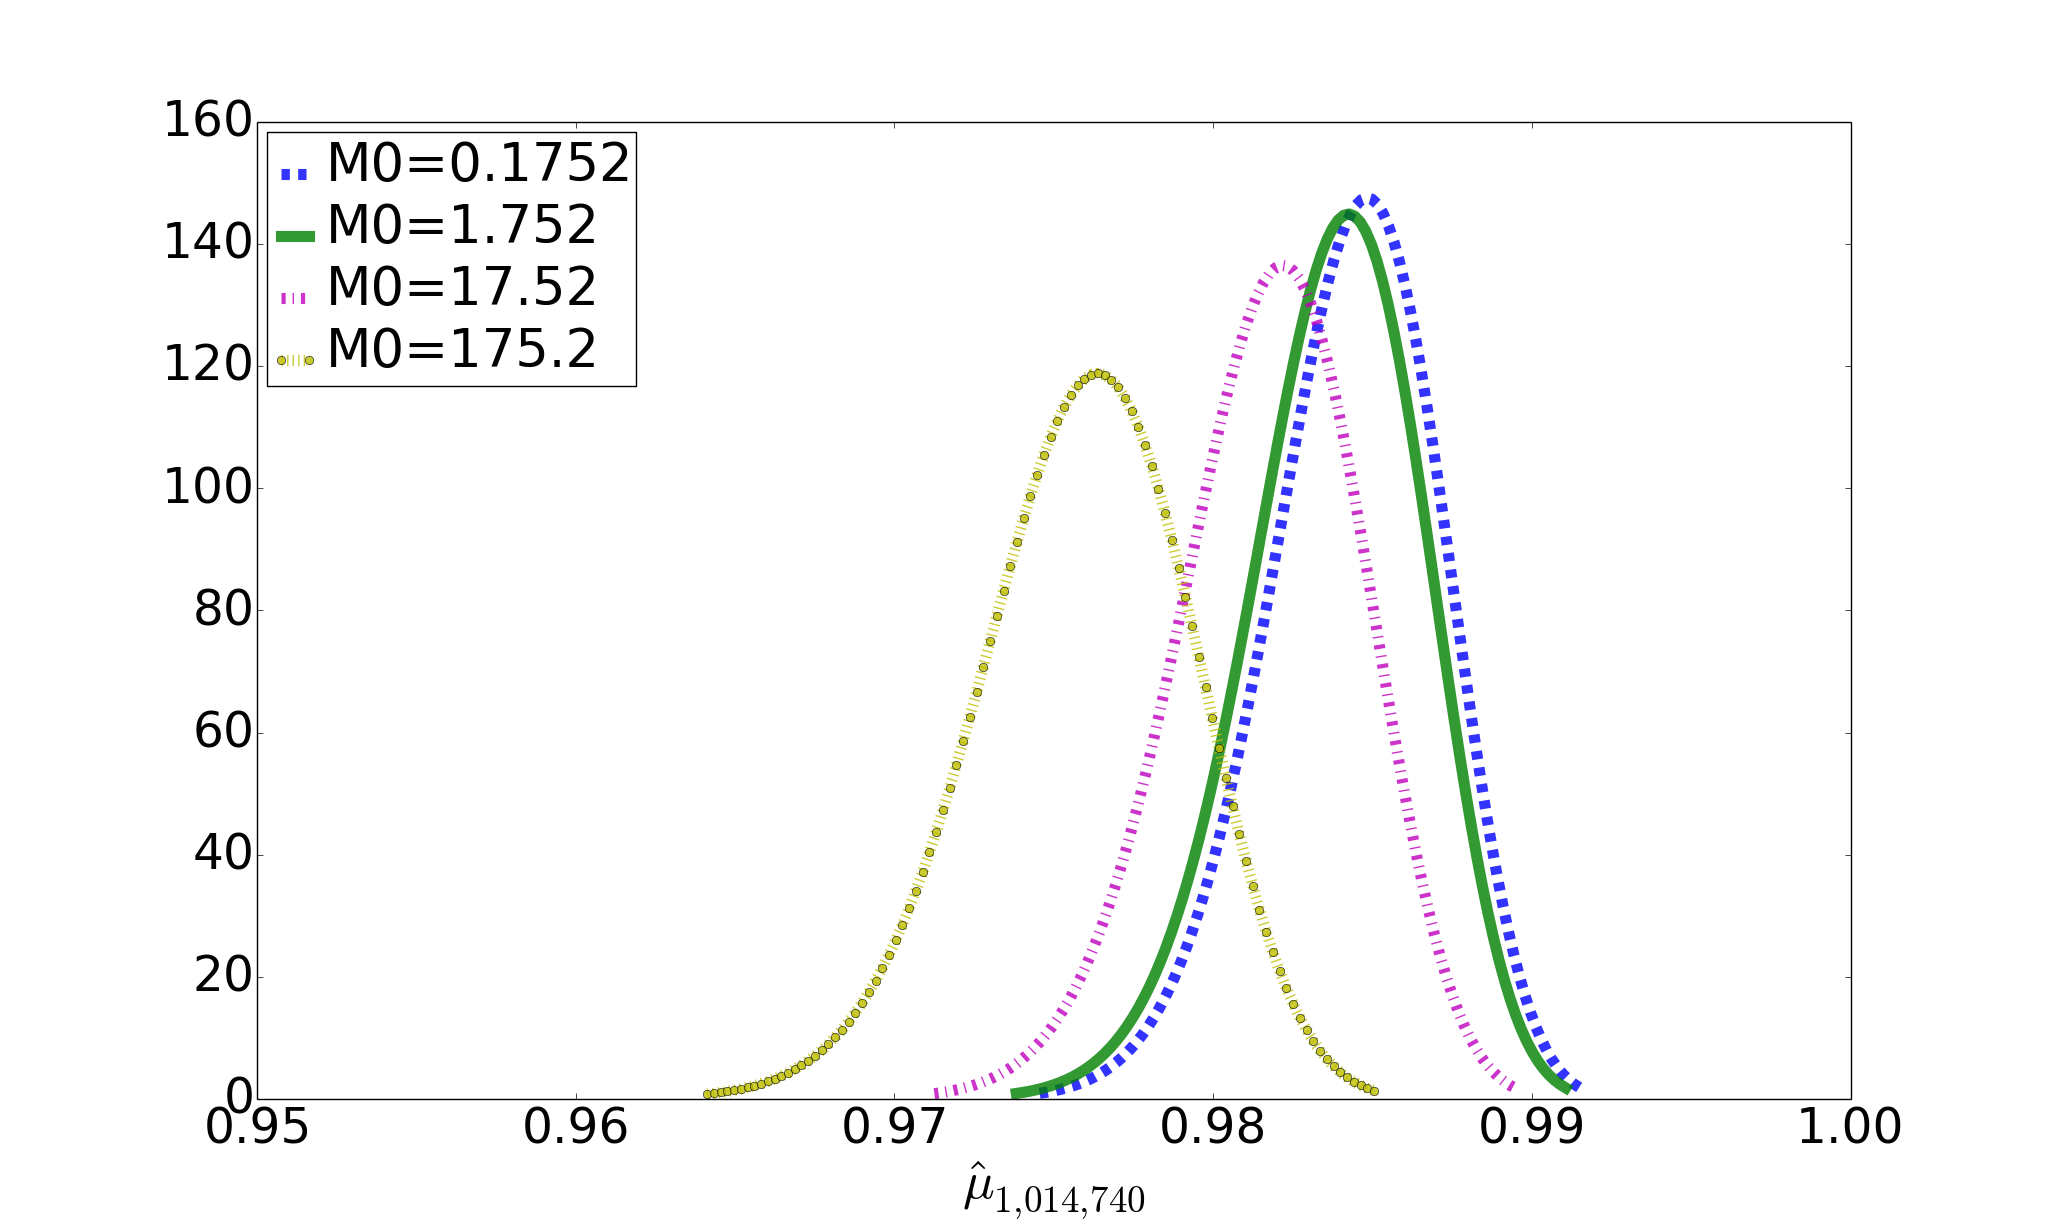
\includegraphics[width=0.8\textwidth]{figs/diff_M0.png}
\caption{Influence of $M_0$ on the estimation of $\mu_j$.
Posterior distributions of variant position 1014740 $\hat{\mu}_{1014740}$ with different $M_0$ are shown.}
\label{tbl:M0}
\end{figure}

% Concomitant variants
We also identified a pair of concomitant variants, Chr04:1014740 in gene MTH1 and Chr12:200286 in gene ADE16, that increase in NRAF together in time (Figure~\ref{tbl:concomitant}).
In this pair of genes, gene MTH1 is a negative regulator of the glucose-sensing signal transduction pathway, and gene ADE16 is an enzyme of $\mathit{de\, novo}$ purine biosynthesis.
Glucose sensing inducts gene expression to help yeast receive necessary nutrients, which could be a reason for this pair of genes to mutate together ~\citep{johnston1999feasting}.
% results are under folder \fzhang\Research\rvd3-variational-notebook\results\2016-01-12_Run_rvd3_Dan_data_regions
\begin{figure}[htbp]
\centering
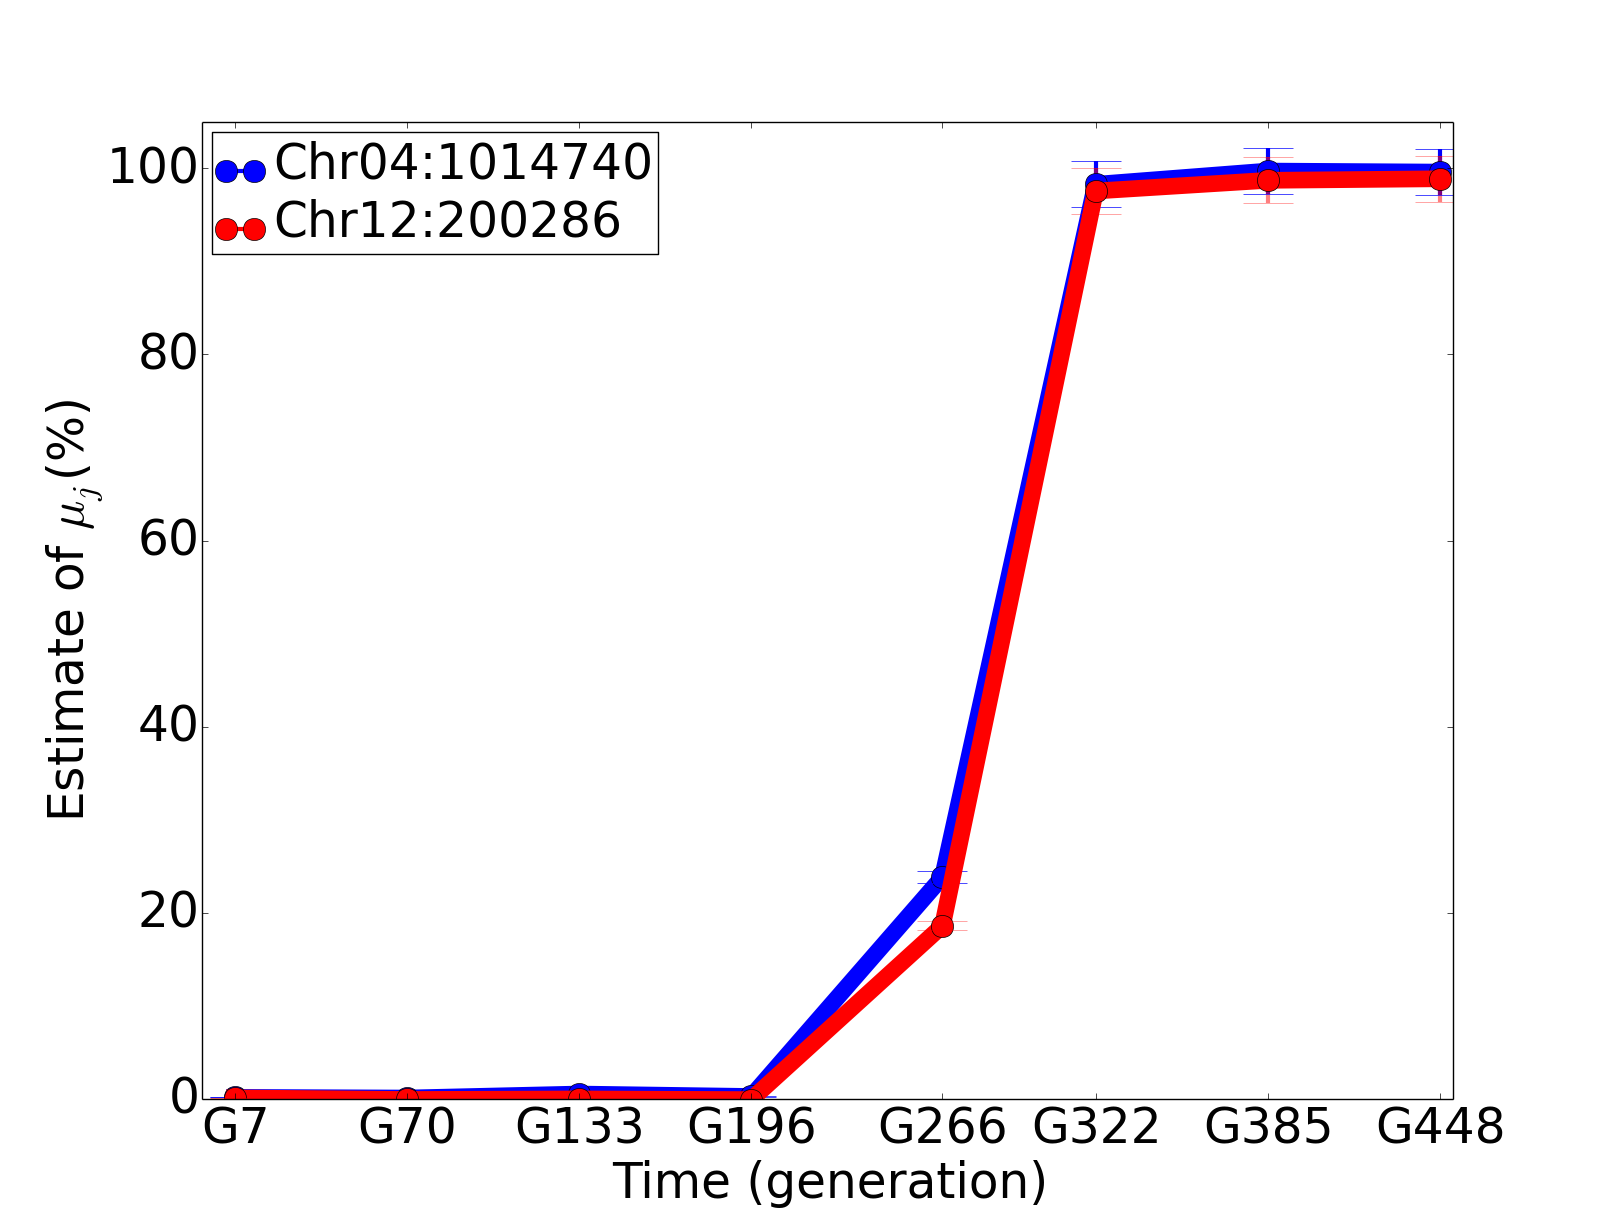
\includegraphics[width=0.65\textwidth]{figs/concomitant.png}
\caption{The NRAF trend of concomitant variants in gene MTH1 and ADE16.
The 95\% Bayesian credible interval are shown.}
\label{tbl:concomitant}
\end{figure}
\section{Discussion}
% Brief summary of RVD3
In this article, we propose a variational EM algorithm to estimate the NRAF by approximating posterior distributions for latent variables.
We derived a variational expectation maximization algorithm to calculate the intractable integration of our Bayesian model.
Our results show that the variational EM algorithm
(i) is able to identify rare variants at a 0.1\% NRAF level with comparable sensitivity and specificity in comparison to a MCMC sampling algorithm;
(ii) has a higher specificity in comparison with many state-of-the-art algorithms in a broad range of NRAFs;
and (iii) detects SNVs early in the evolutionary time course, as well as track the NRAF in a longitudinal yeast data set.

% Potential problems of variational EM and alternative strategies
However, the application on an interested gene region suggests that our variational EM algorithm yields an accurate identification of rare SNVs in sufficient efficiency.
It is possible that the Beta variational distribution we have selected to address the non-conjugate prior issue will not yield the speed improvements as we expect.
In that event, we will instead use a straightforward interpolation scheme to compute the necessary integral for the expectation step.
The Beta function in the integral kernel is relatively smooth and has a bounded domain.
This favorable property can be leveraged to implement a cubic spline interpolation method to approximate the necessary integral ~\citep{mckinley1998cubic}.
Here we aim to guarantee accuracy rather than efficiency, so we calculate the numerical integration without using cost-effective methods.
Another strategy is to consider a Laplace approximation for the proposal variational distribution, as we and others have done previously ~\citep{saddiki2014glad, wang2013variational}.

As a local optimization methodology, variational EM is possible to fall in a local maximum of the variational function.
It could be that the accuracy is not sufficient to identify variants with statistical confidence.
If so, we will generate different random initialized parameters to restart the algorithm.
We can also consider using RVD2 for more accurate posterior approximation, which is implemented by MCMC sampling algorithm.
MCMC is computationally slower, but is easily deployed to multiple computational cores in parallel.
Thus, we will be able to analyze the sequencing data using Amazon Elastic Compute Cloud (EC2) resource, which will increase computational efficiency.

% Future work
The variational EM algorithm discovers many novel variants in the application of an interested region of the longitudinal yeast data set.
These discovered variants drive us to extend our statistical method to the whole genome, whole population yeast sequence data with guaranteed accuracy and efficiency.
By doing this, we can uncover the dynamics of arising variants at the genome-wide scale to show the genetic basis of clonal interference.
Our method is also can be extended to study drug resistance by characterizing tumor heterogeneity in targeted anti-cancer chemotherapy samples.
We will be able to find the causative variants that lead to drug resistance and understand the causes of resistance at the single nucleotide level.
\section{Acknowledgments}
Funding:
%
\appendix
\section{Derivation of the components in ELBO}
\label{appendix:ELBO}
%\section{Derivation of Variational Inference}
%\subsection{Evidence Lower Bound (ELBO)}
Recall that $r_{ij}|n_{ij}\thicksim \text{Binomial}(\theta_{ij}, n _{ji})$,
\begin{equation}
\begin{split}
%\label{r}
E_q \left[ \log p\left(r | \theta, n \right)\right] &= \sum_{j=1}^{J} \sum_{i=1}^{N} E_q  \left[ \log p \left( r_{ji} | \theta_{ji}, n_{ji} \right) \right] \\
&= \sum_{j=1}^{J} \sum_{i=1}^{N}  E_q  \left[ \log \left( \frac{ \Gamma(n_{ji}+1) } { \Gamma(r_{ji}+1) \Gamma( n_{ji} - r_{ji} + 1 ) } \theta_{ji}^{r_{ji}} (1 - \theta_{ji})^{n_{ji} - r_{ji}} \right) \right] \\
&= \sum_{j=1}^{J} \sum_{i=1}^{N} \log \left( \frac{ \Gamma(n_{ji}+1) } { \Gamma(r_{ji}+1) \Gamma( n_{ji} - r_{ji} + 1 ) }\right)  \\
&\quad + \sum_{j=1}^{J} \sum_{i=1}^{N}  E_q  \left[ r_{ji} \log \theta_{ji} + (n_{ji} - r_{ji}) \log (1 - \theta_{ji}) \right] \\
&= \sum_{j=1}^{J} \sum_{i=1}^{N} \log \left( \frac{ \Gamma(n_{ji}+1) } { \Gamma(r_{ji}+1) \Gamma( n_{ji} - r_{ji} + 1 ) }\right)  \\
&\quad + \sum_{j=1}^{J} \sum_{i=1}^{N} \left\lbrace r_{ji} E_q \left[ \log \theta_{ji} \right] + (n_{ji} - r_{ji}) E_q  \left[  \log (1 - \theta_{ji}) \right] \right\rbrace. \\
\end{split}
\end{equation}
Recall that $\mu_j \thicksim \text{Beta}(\mu_0, M_0)$,
\begin{equation}
\begin{split}
%\label{mu}
E_q \left[ \log p\left(\mu ; \mu_0, M_0 \right)\right] &= \sum_{j=1}^{J} E_q  \left[ \log p\left( \mu_j; \mu_0, M_0 \right) \right] \\
&= \sum_{j=1}^{J} E_q  \left[ \log \left( \frac{ \Gamma(M_0) } { \Gamma(\mu_0 M_0) \Gamma(M_0 (1-\mu_0)) } \mu_j^{M_0\mu_0 -1} (1 - \mu_j)^{M_0 ( 1 - \mu_0) - 1} \right) \right] \\
%&= \sum_{j=1}^{J} \log \frac{ \Gamma(M_0) } { \Gamma(\mu_0 M_0) \Gamma(M_0 (1-\mu_0))} \\
%&\quad + \sum_{j=1}^{J} \left\lbrace (M_0\mu_0 -1)E_q  \left[ \log \mu_j \right] + (M_0 ( 1 - \mu_0) - 1) E_q  \left[ \log (1 - \mu_j)\right]\right\rbrace  \\
&= J* \log \frac{ \Gamma(M_0) } { \Gamma(\mu_0 M_0) \Gamma(M_0 (1-\mu_0))} \\
&\quad + \sum_{j=1}^{J} \left\lbrace (M_0\mu_0 -1)E_q  \left[ \log \mu_j \right] + (M_0 ( 1 - \mu_0) - 1) E_q  \left[ \log (1 - \mu_j)\right]\right\rbrace.
\end{split}
\end{equation}
Recall that $\theta_{ji} \thicksim \text{Beta}(\mu_j, M_j)$,
\begin{equation}
\begin{split}
%\label{theta}
E_q \left[ \log p\left(\theta | \mu; M \right)\right] &= \sum_{j=1}^{J} \sum_{i=1}^{N} E_q \left[ \log p\left(\theta_{ji} | \mu_j; M_j \right)\right] \\
&= \sum_{j=1}^{J} \sum_{i=1}^{N}  E_q  \left[ \log \left( \frac{ \Gamma(M_j) } { \Gamma(\mu_j M_j) \Gamma(M_j (1-\mu_j)) } \theta_{ji}^{M_j\mu_j -1} (1 - \theta_{ji})^{M_j ( 1 - \mu_j) - 1} \right) \right] \\
&= \sum_{j=1}^{J} \sum_{i=1}^{N} E_q  \left[ \log \left( \frac{ \Gamma(M_j) } { \Gamma(\mu_j M_j) \Gamma(M_j (1-\mu_j)) }\right) \right] \\
&\quad + \sum_{j=1}^{J} \sum_{i=1}^{N}  E_q  \left[ \log \left( \theta_{ji}^{M_j\mu_j -1} (1 - \theta_{ji})^{M_j ( 1 - \mu_j) - 1} \right) \right] \\
&= \sum_{j=1}^{J} \sum_{i=1}^{N} E_q  \left[ \log \left( \frac{ \Gamma(M_j) } { \Gamma(\mu_j M_j) \Gamma(M_j (1-\mu_j)) }\right) \right]  \\
&\quad + \sum_{j=1}^{J} \sum_{i=1}^{N} \left\lbrace E_q \left[ \left( M_j\mu_j -1 \right) \log \theta_{ji} \right] + E_q \left[ \left( M_j ( 1 - \mu_j) - 1 \right) \log \left( 1 - \theta_{ji} \right) \right]\right\rbrace \\
&= \sum_{j=1}^{J} \sum_{i=1}^{N} E_q  \left[ \log \left( \frac{ \Gamma(M_j) } { \Gamma(\mu_j M_j) \Gamma(M_j (1-\mu_j)) }\right) \right] \\
&\quad + \sum_{j=1}^{J} \sum_{i=1}^{N} \left\lbrace M_j E_q \left[ \mu_j \right] E_q \left[ \log \theta_{ji} \right] - E_q  \left[ \log \theta_{ji} \right] + \left( M_j - 1 - M_j E_q\left[ \mu_j \right]  \right) E_q\left[ \log \left( 1 - \theta_{ji}\right) \right] \right\rbrace \\
&= N* \sum_{j=1}^{J} E_q  \left[ \log \left( \frac{ \Gamma(M_j) } { \Gamma(\mu_j M_j) \Gamma(M_j (1-\mu_j)) }\right) \right] \\
&\quad + \sum_{j=1}^{J} \sum_{i=1}^{N} \left\lbrace M_j E_q \left[ \mu_j \right] E_q \left[ \log \theta_{ji} \right] - E_q  \left[ \log \theta_{ji} \right] + \left( M_j - 1 - M_j E_q\left[ \mu_j \right]  \right) E_q\left[ \log \left( 1 - \theta_{ji}\right) \right] \right\rbrace.
\end{split}
\end{equation}
%
%Therefore, in order to compute ELBO, we need to compute the following expectations with respect to variational distribution:
%
%$ E_q \left[ \log \theta_{ji} \right] $, $ E_q\left[ \log \left( 1 - \theta_{ji}\right) \right] $ , $ E_q  \left[ \log \mu_j \right] $ , $ E_q  \left[ \log (1 - \mu_j)\right] $, $ E_q \left[ \mu_j \right] $, and $ E_q\left[ \log \left( \frac{ \Gamma(M_j) } { \Gamma(\mu_j M_j) \Gamma(M_j (1-\mu_j)) }\right)\right] $.

%\subsection{Variational Distributions}
%\label{appendix:var}
%Given the variational distributions, we have
%\begin{align}
%E_q \left[ \log \theta_{ji} \right] &= \psi(\delta_{ji1}) - \psi(\delta_{ji1}+\delta_{ji2}) \nonumber, \\
%E_q \left[ \log \left( 1 - \theta_{ji}\right) \right]&= \psi(\delta_{ji2}) - \psi(\delta_{ji1}+\delta_{ji2}) \nonumber, \\
%E_q \left[ \mu_j \right] &= \frac{\gamma_{j1}}{\gamma_{j1} + \gamma_{j2}} \nonumber, \\
%E_q  \left[ \log \mu_j \right] &= \psi(\gamma_{j1}) - \psi(\gamma_{j1}+\gamma_{j2}) \nonumber, \\
%E_q  \left[ \log (1 - \mu_j)\right] &= \psi(\gamma_{j2}) - \psi(\gamma_{j1}+\gamma_{j2})\nonumber. \\
%\end{align}
%There is no analytical representation for $  E_q  \left[ \log \Gamma(\mu_j M_j) \right] $ and $ E_q  \left[ \log \Gamma(M_j (1-\mu_j)) \right] $.
%Therefore, we propose to use trapezoidal numerical integration to approximate these two expectations.
%
%Moreover, according to the entropy of beta distribution random variable,
%\begin{equation}
%\begin{split}
%E_q \left[ \log q\left(\mu \right)\right] &= \sum_{j=1}^{J} E_q \left[ \log q(\mu_j)\right] \\
%&= -\sum_{j=1}^{J} \left\lbrace \log (B(\gamma_{j1},\gamma_{j2}))-(\gamma_{j1}-1)\psi(\gamma_{j1})-(\gamma_{j2}-1)\psi(\gamma_{j2})
%+ (\gamma_{j1}+\gamma_{j2}-2)\psi(\gamma_{j1}+\gamma_{j2})\right\rbrace;
%\end{split}
%\end{equation}
%\begin{equation}
%\begin{split}
%E_q \left[ \log q\left(\theta \right)\right] &= \sum_{j=1}^{J}\sum_{i=1}^{N} E_q\left[ \log q(\theta_{ji})\right] \\
%&= -\sum_{j=1}^{J}\sum_{i=1}^{N} \\
%&\quad \left\lbrace \log (B(\delta_{ji1},\delta_{ji2}))-(\delta_{ji1}-1)\psi(\delta_{ji1})-(\delta_{ji2}-1)\psi(\delta_{ji2})
%+ (\delta_{ji1}+\delta_{ji2}-2)\psi(\delta_{ji1}+\delta_{ji2})\right\rbrace.
%\end{split}
%\end{equation}

%\subsection{Optimizing Model Parameters} % $ \phi = \left\lbrace \mu_0, M_0, M \right\rbrace  $}
%\label{appendix:para}
%% Optimizing mu0
%\subsubsection{Optimizing $ \mu_0 $}
%The ELBO with respect to $ \mu_0 $ is
%\begin{equation}
%\begin{split}
%\label{mu_0}
%\mathcal{L}_{[\mu_0]}
%&= -J*\log  \Gamma(\mu_0 M_0) - J*\log \Gamma(M_0 (1-\mu_0))
%+ M_0\mu_0\sum_{j=1}^{J} \left\lbrace E_q  \left[ \log \mu_j \right]
%- E_q  \left[ \log (1 - \mu_j)\right]\right\rbrace . \\
%\end{split}
%\end{equation}
%Take the derivative with respect to $ \mu_0 $ and set it equal to zero,
%\begin{equation}
%\begin{split}
%\label{mu_0}
%\mathcal{L}_{[\mu_0]}'
%&= -J*M_0 \psi(\mu_0 M_0) + J*M_0 \psi(M_0 (1-\mu_0))
%+ M_0\sum_{j=1}^{J} \left\lbrace E_q  \left[ \log \mu_j \right]
%- E_q  \left[ \log (1 - \mu_j)\right]\right\rbrace =0 , \\
%\end{split}
%\end{equation}
%the update for $ \mu_0 $ can be numerically computed.
%% Optimizing M0
%\subsubsection{Optimizing $ M_0 $}
%The ELBO with respect to $ M_0 $ is
%\begin{equation}
%\begin{split}
%\label{M_0}
%\mathcal{L}_{[M_0]}
%&=J* \log \frac{ \Gamma(M_0) } { \Gamma(\mu_0 M_0) \Gamma(M_0 (1-\mu_0))}
%+ M_0 \sum_{j=1}^{J} \left\lbrace \mu_0E_q  \left[ \log \mu_j \right] + ( 1 - \mu_0) E_q  \left[ \log (1 - \mu_j)\right]\right\rbrace.  \\
%\end{split}
%\end{equation}
%Take the derivative with respect to $ M_0 $ and set it equal to zero,
%\begin{equation}
%\begin{split}
%\label{M_0}
%\mathcal{L}_{[M_0]}'
%&= \log \frac{ \Gamma(M_0) } { \Gamma(\mu_0 M_0) \Gamma(M_0 (1-\mu_0))}
%+ M_0 \sum_{j=1}^{J} \left\lbrace \mu_0E_q  \left[ \log \mu_j \right] + ( 1 - \mu_0) E_q  \left[ \log (1 - \mu_j)\right]\right\rbrace  \\
%&= \psi(M_0)  - \mu_0 \psi(\mu_0 M_0) - (1-\mu_0) \psi(M_0 (1-\mu_0))  \\
%\quad &+ \sum_{j=1}^{J} \left\lbrace \mu_0E_q  \left[ \log \mu_j \right] + ( 1 - \mu_0) E_q  \left[ \log (1 - \mu_j)\right]\right\rbrace \\
%&=0, \\
%\end{split}
%\end{equation}
%the update for $ M_0 $ can be numerically computed.
%% Optimizing M
%\subsubsection{Optimizing $ M $}
%\begin{equation}
%\begin{split}
%%\label{M}
%\mathcal{L}_{{[M]}}
%&= \sum_{j=1}^{J} E_q  \left[ \log \left( \frac{ \Gamma(M_j) } { \Gamma(\mu_j M_j) \Gamma(M_j (1-\mu_j)) }\right) \right] \\
%&\quad + M_j \sum_{j=1}^{J} \sum_{i=1}^{N} \left\lbrace E_q \left[ \mu_j \right] E_q \left[ \log \theta_{ji} \right] + \left( 1 - E_q\left[ \mu_j \right]  \right) E_q\left[ \log \left( 1 - \theta_{ji}\right) \right] \right\rbrace \\
%\end{split}
%\end{equation}
%Suppose
%\begin{equation}
%\begin{split}
%f(\mu) &= \log\left( \frac{\Gamma(M)}{\Gamma(\mu M) \Gamma(M (1-\mu ))}\right) \nonumber, \\
%\end{split}
%\end{equation}
%then
%\begin{align}
%f'(\mu) &= -M \psi (\mu M) + M \psi(M (1-\mu )) \nonumber \\
%f''(\mu) &= -M^2 \psi ' (\mu M) - M^2 \psi '(M (1-\mu )) <0 \nonumber, \\
%\end{align}
%where $ \psi(\mu) $ is the Digamma function, and $ \psi'(\mu)= \frac{\partial \psi(\mu)}{\partial \mu}$ is the Trigamma function. As trigamma function $ \psi'(\mu) $ is positive, $ f''(\mu) $ is negative.
%Thus, $ f(\mu) $ is a concave function.
%We can approximate $ f(\mu) $ using first-order Taylor expansion around point $ \mu^{\circ} $, which is
%\begin{equation}
%\begin{split}
%%f(\mu) &\geq f(\mu_0) + f'(\mu_0) \cdot (\mu-\mu_0) \nonumber \\
%%&= \log\left( \frac{\Gamma(M)}{\Gamma(\mu_0 M) \Gamma(M (1-\mu_0 ))}\right) + \left( -M \psi (\mu_0 M) + M \psi(M (1-\mu_0 ))\right) \cdot (\mu-\mu_0)
%f(\mu) &\leq f(\mu^{\circ}) + f'(\mu^{\circ}) \cdot (\mu-\mu^{\circ}) \nonumber \\
%&= \log\left( \frac{\Gamma(M)}{\Gamma(\mu^{\circ} M) \Gamma(M (1-\mu^{\circ} ))}\right) + \left( -M \psi (\mu^{\circ} M) + M \psi(M (1-\mu^{\circ} ))\right) \cdot (\mu-\mu^{\circ}).
%\end{split}
%\end{equation}
%%
%A upper bound approximation for $ E_q  \left[ \log \left( \frac{ \Gamma(M_j) } { \Gamma(\mu_j M_j) \Gamma(M_j (1-\mu_j)) }\right) \right] $ around point $ \mu_j^{\circ} $ can be represented as
%\begin{equation}
%\begin{split}
%E_q  \left[ \log \left( \frac{ \Gamma(M_j) } { \Gamma(\mu_j M_j) \Gamma(M_j (1-\mu_j)) }\right) \right] &\leq \log\left( \frac{\Gamma(M_j)}{\Gamma(\mu_j^{\circ} M_j) \Gamma(M_j (1-\mu_j^{\circ} ))}\right) \\
%\quad &+ \left( -M_j \psi (\mu_j^{\circ} M_j) + M_j \psi(M_j (1-\mu_j^{\circ} ))\right) \cdot (E_q(\mu_j)-\mu_j^{\circ}).\nonumber
%\end{split}
%\end{equation}
%%
%The equality holds if and only if $ \mu_j^{\circ} =E_q(\mu_j) $.
%Therefore, at this particular point,
%\begin{equation}
%\begin{split}
%E_q  \left[ \log \left( \frac{ \Gamma(M_j) } { \Gamma(\mu_j M_j) \Gamma(M_j (1-\mu_j)) }\right) \right] &= \log\left( \frac{\Gamma(M_j)}{\Gamma(E_q(\mu_j) M_j) \Gamma(M_j (1-E_q(\mu_j) ))}\right).\nonumber
%\end{split}
%\end{equation}
%%
%Then
%\begin{equation}
%\begin{split}
%%\label{M}
%\mathcal{L}_{{[M]}}
%&= \sum_{j=1}^{J} \log\left( \frac{\Gamma(M_j)}{\Gamma(E_q(\mu_j) M_j) \Gamma(M_j (1-E_q(\mu_j) ))}\right) \\
%&\quad + M_j \sum_{j=1}^{J} \sum_{i=1}^{N} \left\lbrace E_q \left[ \mu_j \right] E_q \left[ \log \theta_{ji} \right] + \left( 1 - E_q\left[ \mu_j \right]  \right) E_q\left[ \log \left( 1 - \theta_{ji}\right) \right] \right\rbrace. \\
%\end{split}
%\end{equation}
%%
%The partial derivative is
%\begin{equation}
%\begin{split}
%\frac{\partial \mathcal{L}_{{[M]}} }{\partial \ M_j}
%&= \psi(M_j) - E_q(\mu_j) \psi(E_q(\mu_j) M_j)
%- (1-E_q(\mu_j)) \psi((1-E_q(\mu_j)) M_j) \\
%&\quad + \sum_{j=1}^{J} \sum_{i=1}^{N} \left\lbrace E_q \left[ \mu_j \right] E_q \left[ \log \theta_{ji} \right]
%+ \left( 1 - E_q\left[ \mu_j \right]  \right) E_q\left[ \log \left( 1 - \theta_{ji}\right) \right] \right\rbrace, \\
%\end{split}
%\end{equation}
%%
%the update for $ M_j $ can be numerically computed.


\bibliographystyle{named}
\bibliography{ref}

\end{document}
